\documentclass{article}

% formatting
\usepackage[utf8]{inputenc} % allow utf-8 input
\usepackage[T1]{fontenc} % use 8-bit T1 fonts  (allows for direct use of ö,ü,etc.)

% math typesetting
\usepackage{amsmath}
\usepackage{amssymb}
\usepackage{amsfonts}

% maths definitions, theorems, etc.
\usepackage{amsthm}

% color
\usepackage{color}
\usepackage{xcolor}

% layout
\usepackage{layout}
\usepackage{lipsum}

% cross-referencing and hyperlinks
\usepackage{hyperref}
\usepackage{url}
\usepackage{doi}

% figures
\usepackage{graphicx}
\usepackage{subfig}
\usepackage{wrapfig}

% tables
\usepackage{booktabs}
\usepackage{multirow}
\usepackage{caption} 
\usepackage{float}

% enumeration
\usepackage{enumitem}

% embedding pages
\usepackage{pdfpages}

% multi-line comments
\usepackage{comment}

% landscape orientation
\usepackage{rotating}
\usepackage{pdflscape}

% Gantt charts
\usepackage{pgfgantt}

% footnotes
\usepackage{footnote}

% code
\usepackage{listings}

% matrices and tables
\usepackage{nicematrix}
\usepackage{varwidth}
% \usepackage{tabularx} do not load package tabularx, instead use package nicematrix

% document structure
\setcounter{secnumdepth}{5} % enable numbered sub-sub-sections etc.

% custom header size
\usepackage{titlesec}

% customized references (make "Figure 1" a link, not just "1")
\usepackage[capitalise, nameinlink]{cleveref}

% customized frames around text etc.
\usepackage{mdframed}

% tikz
\usepackage{tikz}

% calligraphy
\usepackage{calligra}

% chemical formulas
\usepackage{chemformula}
% column layout
\usepackage{multicol}
\setlength{\columnsep}{0.75cm}

% paragraphs
\usepackage[skip=0.5\baselineskip]{parskip}

% geometry
\usepackage[
    margin = 3cm,
    top = 3cm,
    bottom = 3cm
]{geometry}

% header size
\titleformat*{\section}{\large\bfseries}%{\thesection.}{\hspace{0cm}}{}
\titleformat*{\subsection}{\normalsize\bfseries}%{\thesection.}{\hspace{0cm}}{}
\titleformat*{\subsubsection}{\normalsize\bfseries}
\titleformat*{\paragraph}{\normalsize\bfseries}
\titleformat*{\subparagraph}{\normalsize\bfseries}

% custom headers
\usepackage{fancyhdr}
\pagestyle{fancy} % custom headers and footers
\setlength{\headheight}{15pt} % height of header
\setlength{\headsep}{10pt} % separation between header and main text

\usepackage[
    backend=biber,
    style=ieee
]{biblatex}
\addbibresource{references.bib}
% show DOI URL (https://doi.org/XXX.XXXXX.XXXX), instead of publisher URL (https://springer.com/XXXX)
% cf. https://tex.stackexchange.com/a/616241
\DeclareSourcemap{
  \maps[datatype = bibtex]{
    \map{
      \step[notfield = keywords, final]
      \step[fieldsource = doi, final]
      \step[fieldset = url, null]
    }
    \map{
      \step[fieldsource = keywords, notmatch = \regexp{\bprimary\b}, final]
      \step[fieldsource = doi, final]
      \step[fieldset = url, null]
    }
  }
}
\AtEveryBibitem{
    \clearfield{urlyear}
    \clearfield{urlmonth}
}

\renewcommand{\contentsname}{\centering Contents} % https://tex.stackexchange.com/a/308207
\usepackage[titles, subfigure]{tocloft} % https://tex.stackexchange.com/a/336618
\renewcommand{\cftsecleader}{\cftdotfill{\cftdotsep}} % https://tex.stackexchange.com/a/271942


\usepackage{tikz}


\newcommand{\ExternalLink}{%
    \tikz[x=1.2ex, y=1.2ex, baseline=-0.05ex]{% 
        \begin{scope}[x=1ex, y=1ex]
            \clip (-0.1,-0.1) 
                --++ (-0, 1.2) 
                --++ (0.6, 0) 
                --++ (0, -0.6) 
                --++ (0.6, 0) 
                --++ (0, -1);
            \path[draw, 
                line width = 0.5, 
                rounded corners=0.5] 
                (0,0) rectangle (1,1);
        \end{scope}
        \path[draw, line width = 0.5] (0.5, 0.5) 
            -- (1, 1);
        \path[draw, line width = 0.5] (0.6, 1) 
            -- (1, 1) -- (1, 0.6);
        }
    }

%%%%%%%%%%%%%%%%%%%%%%%%%%%%%%%%%%%%%%%%%%%%%%%%%%%%%%%%%%%%%%%%%%%%%

% document metadata
\title{Proposal for a Summer Academy}
\author{Michael P. Weinold$^1$, Philippe Schultheiss$^1$, Mark C. Ballandies$^2$}
\date{
    $^1$Schweizerische Studienstiftung \\
    $^2$Studienstiftung des Deutschen Volkes \\[3mm]
    October 2023
}

%%%%%%%%%%%%%%%%%%%%%%%%%%%%%%%%%%%%%%%%%%%%%%%%%%%%%%%%%%%%%%%%%%%%%

\begin{document}

\maketitle

\section*{\centering Authors}

\textbf{\textit{Michael P. Weinold}} (born 1995 in Innsbruck, Austria) is a doctoral researcher at ETH Zurich and the Paul Scherrer Institute. His background is in engineering physics, with degrees from Vienna University of Technology and ETH Zurich. His current research is focused on accelerating innovation in novel clean-energy technologies. He builds mathematical models and open-source software to better help decision makers assess the environmental impact of different techno-economic scenarios for decarbonizing the economy. Since 2023, he is a guest lecturer at the Department of Mechanical Engineering of ETH Zurich, where he teaches the introductory unit of the lecture series on \textit{Sustainability and Management of Air Transport}. His interest in aesthetics in the built environment was sparked during his research at the University of Cambridge, where he was introduced to the legacy of the late British philosopher Sir Roger Scruton. Since that time, he has been most interested in how new neuro-scientific insights can enable citizen movements to positively shape public spaces.

\textbf{\textit{Philippe Schultheiss}} (born 1984 in Basel, Switzerland) is a consultant and soon-to-be pastor in the Swiss Reformed Church. He holds an undergraduat degrees in Business \& Economics from the university of Basel as well as a master's degree in Philosophy from the university of Freiburg i.Ue. He is now an alumnus of the Swiss Study Foundation, where he is still engaged as a member of the Assessment Jury as well as a frequent co-organizer of events. He has been interested in politics, especially the areas of environmental and urban planning, since his days at the cantonal school at Schaffhausen. He went on to co-found the Green-Liberal Party in the canton of Schaffhausen and remained involved in local politics after his relocation to Zurich, where, in 2020, he was elected president of the Parliament of the Reformed Church Zurich. This community of more than 70'000 members administers dozens of church buildings. Some of those buildings have already repurposed, and many more of them are expected to find new usages. Hence his motivation to contribute to a prospective and socially beneficial real estate strategy.

\textbf{\textit{Mark C. Ballandies}} (born 1991 in Burgwedel, Germany) is a postdoctoral researcher in the Computational Social Science group at ETH Zurich, where he is exploring decentralised, bottom-up and community-owned solutions to complex challenges, which he is putting into practice with WiHi, a decentralised physical infrastructure network (DePIN) that uses web3 to improve weather and climate predictions. Here he investigates how value-sensitive design - the early incorporation of stakeholder values into the system design process - influences cryptoeconomic incentives and human behaviour.
He is co-founder of DAOSuisse, lecturer at the Vorarlberg University of Applied Sciences, alumnus of the Foundation of German Business, president of education matters e.V., member of the dcent group, initiator of the Smarte Dörfer association.
Mark discovered the beauty of old farmhouses and their effectiveness in combating environmental challenges when he began restoring a half-timbered house from 1870 in 2019, using ecological, locally sourced and recyclable building materials such as wood, clay and hemp. He found that these farmhouses integrate values such as circularity, sustainability and locality into all aspects and details of their design and construction, resulting in unique, sustainable and liveable architectural works. This discovery inspires him in his daily work, which he enjoys sharing with others.


\clearpage

\tableofcontents

\section*{\centering Administrative Information}

\begin{NiceTabularX}{\textwidth}{llX}
\textit{Author} & \textit{Email} & \textit{Phone} \\
\hline
Michael P. Weinold & \texttt{michael@weinold.ch} & \texttt{+41 75 500 70 70} \\
Philippe Schultheiss & \texttt{phschultheiss@protonmail.ch} & \texttt{+41 79 768 53 15} \\
Mark C. Ballandies & \texttt{markballandies@googlemail.com} & \texttt{+41 78 899 87 85}
\end{NiceTabularX}

\begin{NiceTabularX}{\textwidth}{lllX}
\textit{Revision} & \textit{Date} & \href{https://github.com/michaelweinold/latex_swiss_study_foundation}{\textit{Hash} \ExternalLink} & \textit{Comment }\\
\hline
1 & 12.10.2023 & \texttt{c57f656} & First full draft, sent out for feedback to PS and MCB
\end{NiceTabularX}

\section*{\centering Foreword}

The present proposal has been a long time in the making. The idea was born back in October 2021 when the Swiss Study Foundation first opened a call for proposals for the Summer Academies. Only now did all of the authors find the time to commit to the time-consuming creative process that was still required to frame the topic, select potential speakers and draft a schedule for the event.

During the development this proposal, the authors deemed it necessary to collect their thoughts in a structured way. While the authors are aware that the call for proposals from August 2023 only called for a short description of the contents, they decided to embed this into a document providing additional context. The authors further believe the topic of this proposal is not only timely but of an international scope. English has therefore been adopted as the working language of the proposal.

\cref{sec:construction} - \cref{sec:biophilic} provide the context which has inspired the authors to develop the present proposal. A concise formulation is additionally provided in \cref{sec:abstract}. The proposed schedule as well as additional information on the associated speakers is listed in \cref{sec:schedule}. 

\clearpage
\section{\centering Abstract}
\label{sec:abstract}

\begin{minipage}{0.55\textwidth}

    We must reduce global carbon emissions dramatically. The construction sector is responsible for XX\% of annual global carbon emissions. In Switzerland, it accounts for XX\% of carbon emissions (including imported carbon). This number is expected to increase to XX\% in 2050, due to strong immigration.
    
    What is more, the construction sector is notoriously difficult to decarbonise. Together with certain heavy industry sectors and aviation, it is classified as a "hard to abate" sector.
    
    Work is ongoing on decreasing the carbon footprint of building during the construction phase and during the use phase. This includes novel methods for cement, concrete and steel production or the increasing digitisation of buildings ("smart home"). However, there are currently no efforts to increase the lifetime of buildings. In Switzerland, like in the surrounding EU countries, average building lifetime is around 50 years only.
    
    The carbon emissions incurred during new construction of a building vs the refurbishment can be recouped over a period of between XX-XX years. Studies exist for the nordic countries, where the energy cost of non-refurbished buildings is highest. Average building lifetimes are between 50 years (France, with source) and 60 years (Switzerland, with source).
    
    Despite efforts to improve recycling in construction, recycling rate of modern building materials (steel, concrete, glass) remains low (check for source).
    
    [Figure from Crawford on cumulative embodied energy]
    
    At the same time, changing use requirements meet the modernist credo "form follows function". Changing family structures mean that apartments can be ever more compact.
    
    All this amounts to large scale new construction, the majority of which is in the 'modernist' or contemporary style.
    
    Every poll to date has shown that this style is at the very least moderately unpopular with people. Empirical evidence is mounting, thereby providing proof for something that has been well-known to the general public for a long time: "Why is the Modern World So Ugly?" (Alain de Boton)

\end{minipage}\hspace{15mm}
\begin{minipage}{0.35\textwidth}
    \begin{figure}[H]
    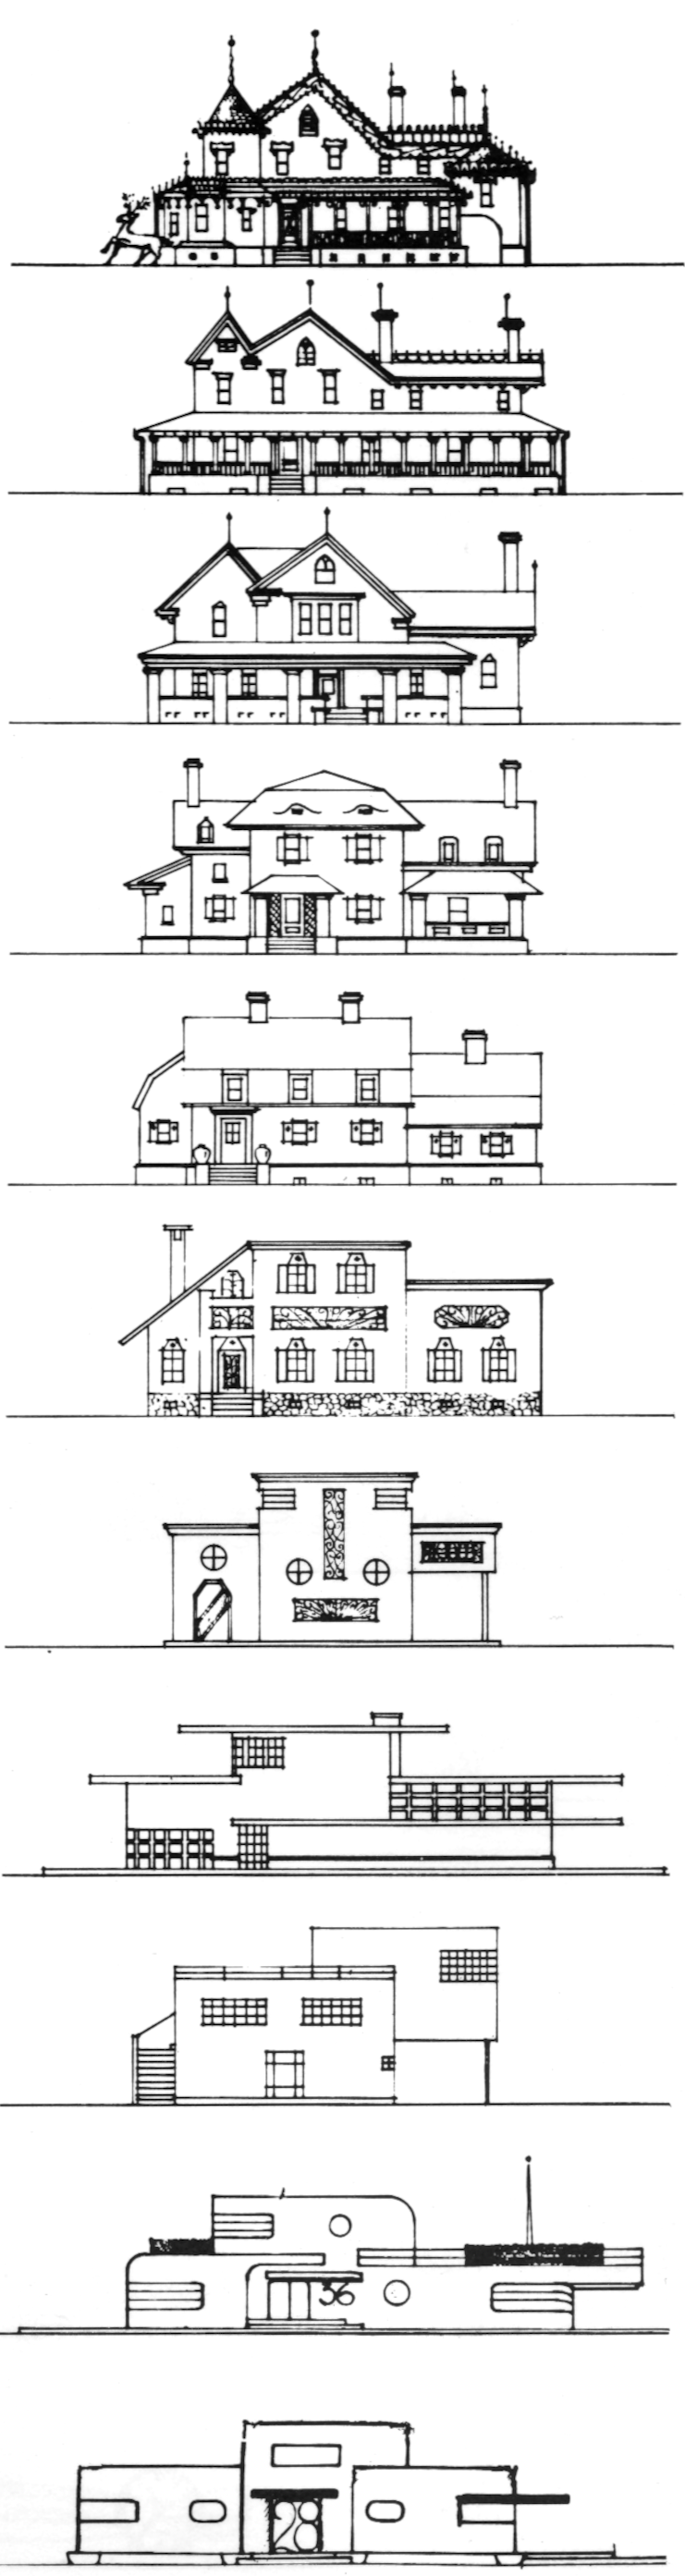
\includegraphics[width=50mm]{./figures/loewy_architecture.png}
    \caption{
        "Design Evolution 1930" by French-born American industrial designer Raymond Loewy \cite{loewy_industrial_1979}
    }
    \label{fig:loewy}
    \end{figure}
\end{minipage}

\clearpage
\section{The Age of Construction}
\label{sec:construction}

\begin{multicols}{2}

Recent data collected by the International Energy Agency shows that the construction of new buildings is expected to add a floor area equivalent to the surface of the city of Paris every week all the way through 2050 \cite[Sec. 3.7]{cozzi_net_2021}.

At the same time, the urban planning offices of several European countries expect and plan for an average service life of newly constructed buildings on the order of only 50 years. The exact lifetime depends on a number of factors, including the purpose of the structure (data for Denmark: 100 years for single-family homes, 75 years for cultural buildings and 50 years for health or teaching buildings \cite{andersen_lifespan_2023}). Further significant differences between the age of the building stock between different countries exist, with buildings in France having a significantly shorter lifetime \cite{noauthor_value_2013} than those in Switzerland \cite{kornmann_service_2012}.

An in-depth investigation of the underlying reasons for the short service life of the majority of the building stock remains an area of active research. In the context of this proposal, we will mention only two:

First, the changing demand structure in the context of residential buildings.

Ongoing societal transformations have driven a continuing trend towards fewer children per family and an increase of single-person households. This trend is illustrated in \cref{fig:households}. New construction of residential buildings is therefore seen as an opportunity to increase urban density by catering to smaller households, avoiding often equally expensive large-scale structural modifications of existing building stock. This trend is so significant that despite low birth rates in industrialized nations, the number of households has grown significantly, even without accounting for migration \cite{noauthor_why_2014}.

It should be noted that the degree of bi-directional causality between an increasing supply of smaller dwellings and family size at the advanced state of this trend has not been conclusively investigated \cite{kulu_fertility_2007}. For instance, the 2021 edition of the U.S. Census Bureau American Community Survey showed fertility rates for occupants of single-family homes to be significantly larger than occupants of apartment buildings \cite{noauthor_american_2021}. Decreasing the supply of larger dwellings on the housing market could induce a feedback loop, whereby the decreasing space of apartments decreases statistical fertility, necessitating even more new construction.

\end{multicols}

\begin{figure}[ht!]
    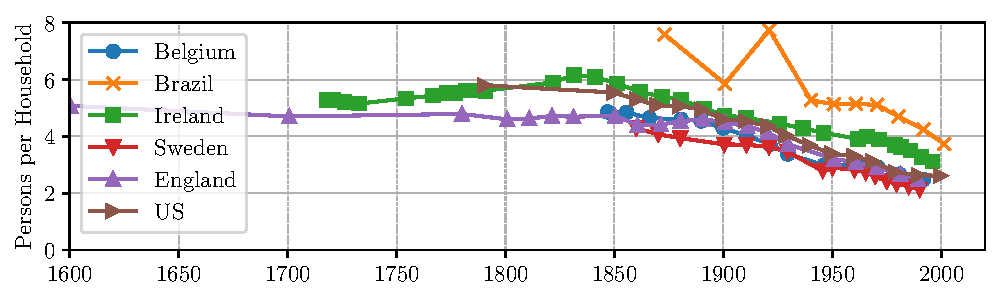
\includegraphics[width=\textwidth]{./figures/household_size.pdf}
    \vspace{-5mm}
    \caption{
        Average household size for different countries between 1600 and 2000. Each point represents average household size during the census for the corresponding year. The figure illustrated how the average number of people living in a household has been shrinking in developed countries for centuries, with the pace of this change accelerating in the early 1900s. A statistical analysis of the data by the authors of the original study shows 
        a significant change in the trend of household size for developed nations around the year 1893. The authors concluded: \textit{"the number of households grew faster than population size in every country and every time period."}. Figure source: Own rendering, with data adapted Mason et al. \cite[Figure 2]{bradbury_long-term_2014}
    }
    \label{fig:households}
\end{figure}

\clearpage
\begin{multicols}{2}

Second, the "diminishing climate returns" of extending building service-life.

The construction and maintenance of buildings in 2022 was responsible for 40\% of global carbon emissions \cite{camarasa_energy_2023}. Consequently, policy makers have been focusing on \textit{"accelerating and rapidly scaling up energy efficiency measures"} in the construction sector \cite{noauthor_2022_2022}. Researchers of the Intergovernmental Panel on Climate Change (IPCC) Working Group for Climate Change Mitigation in recently re-affirmed the emissions reduction potential that the sector offered. Proposed measures include improving existing buildings efficiency and use, high-performance new buildings, integrating renewable energy production in buildings, and decarbonizing production of building materials \cite{shukla_mitigation_2022}.

In this context, the energy expenditure and associated carbon emissions of the construction sector have recently come under increasing scrutiny from researchers in the field of industrial ecology, life-cycle assessment and sustainable construction \cite{chau_review_2015}\cite{ortiz_sustainability_2009}. A key finding is illustrated in \cref{fig:energy}: While extending the lifetime of buildings decreases the carbon emissions associated with its use, this effect naturally decreases over the lifetime of the building, as the recurrent carbon emissions from necessary refurbishment accumulate. Constructing an entirely new building to higher energy efficiency standards is therefore often seen as the preferable option for buildings over a certain age.

This, of course, is in contrast to World Green Building Council: \textit{"The most sustainable building is ironically, the one not built"}

\textit{"Reducing the use of high-volume, carbon-intensive materials such as concrete, steel and plastics, and replacing them with low-carbon and circular alternatives, should be the main approach."} \cite[Sec. 7.4]{noauthor_2022_2022}

Ultimately, many proposed to decarbonize the economy are challenging for technical and political reasons. This includes a reduction of personal mobility, additional taxes on flights or the electrification of sectors with \textit{hard to abate} carbon emissions. At the same time, some of the most straightforward pathways remain unexplored - for instance: \textit{"Don't design houses for a 50 year service life."}.

\end{multicols}

\begin{figure}[ht!]
    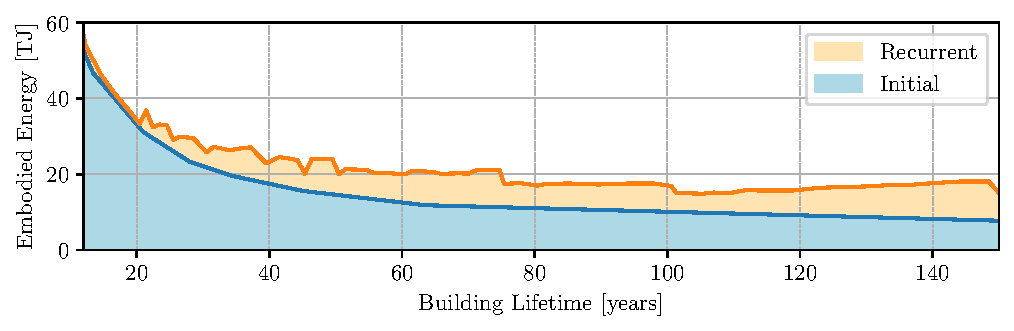
\includegraphics[width=\textwidth]{./figures/building_embodied_energy.pdf}
    \vspace{-5mm}
    \caption{
        Life-cycle embodied energy of a single-storey detached house by building service life. The functional unit of the assessment is the provisioning of the case-study building over a period of 150 years. A building lifetime of 15 years assumes that the house is torn down and rebuilt 10 times during the 150 year investigated timeframe. In this case, the figure show that the majority of energy is expended on the reconstruction ("initial"). On the other hand, a building lifetime of 150 years assumes that house is never torn down in the investigated timeframe. In this case, the figure shows that the majority of the energy is expended on refurbishment and renovation ("recurrent").
        \newline Figure source: Own rendering, with data adapted from Rauf and Crawford \cite[Figure 5]{rauf_building_2015}
    }
    \label{fig:energy}
\end{figure}

\clearpage
\section{The Age of Ugliness}
\label{sec:ugliness}

\begin{multicols}{2}
    
The Swiss-British philosopher Alain de Botton of \textit{"School of Life"} fame in 2021 published an essay titled \textit{"Why is the modern world so ugly?"} \cite{howarth_why_2021}.  likens the development of modern architectural aesthetics to a “war on beauty”, in which a supposedly objective standard of attractiveness has been sacrificed at the altar of originality, resulting in built landscapes that not only violate their inhabitants’ supposedly natural sense of organic beauty but also assault their mental wellbeing. The essay communicated ideas that Botton had developed in an earlier book \textit{"The Architecture of Happiness"}. The essay was promptly decried by \cite{rogan_trads_2021}, without presenting substantive evidence against Botton's main claims: That the majority of modern architecture was widely rejected by the general public. 

This case-study replicates an established pattern in the present architectural community. Mounting evidence that the majority of buildings is perceived as \textit{ulgy}, or at the very least \textit{not beautiful} by the public, followed by calls of architects to ignore the vulgar tastes of the public. 

Three large-scale polls on architectural preferences have been conducted during the past ten years, all replicating the same result. A poll conducted by YouGov in the United Kingdom (sample size $>$1000) \cite{noauthor_yougov_2009}, a poll conducted by The Harris Poll in the United States (sample size $>$2000) \cite{noauthor_americans_2020} and a poll conducted by the Center for Urban and Real Estate Management of the University of Zurich (sample size $>$2000) \cite{hollenstein_schone_2022} \footnote{It should be noted that despite the best efforts of the authors, no scientific study or poll was found that provided evidence to the contrary. Without any claim to completeness, we can therefore say XXXXX}.

Shown in \cref{fig:federal_buildings} is a sample from the U.S. poll.




As we have seen illustrated in the proclamations of Corbusier and XXX, "Taste is subjective" (and we must take part in) has always been the the refuge of modernists. Corbusier said that the public had to be re-educated, and others have wondered about the vulgarity of designs for the public and asked whether architects should take these architectural tastes seriously.

\end{multicols}

\begin{figure}[ht!]
    \centering
    \subfloat{{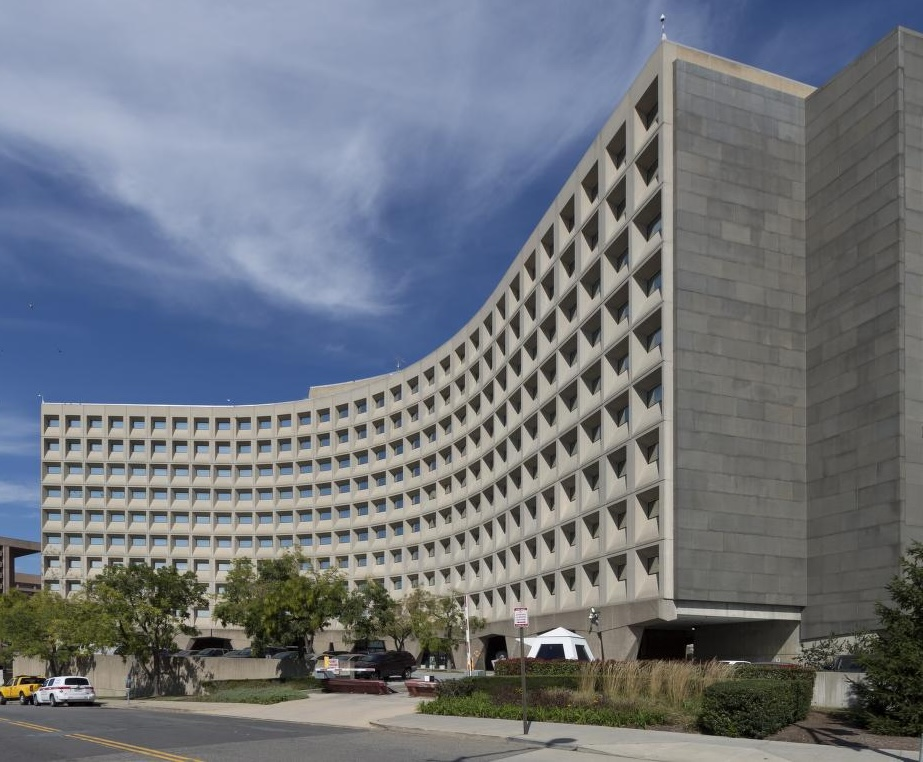
\includegraphics[height=5cm]{figures/us_gov_modernist_1.jpg} }}
    \subfloat{{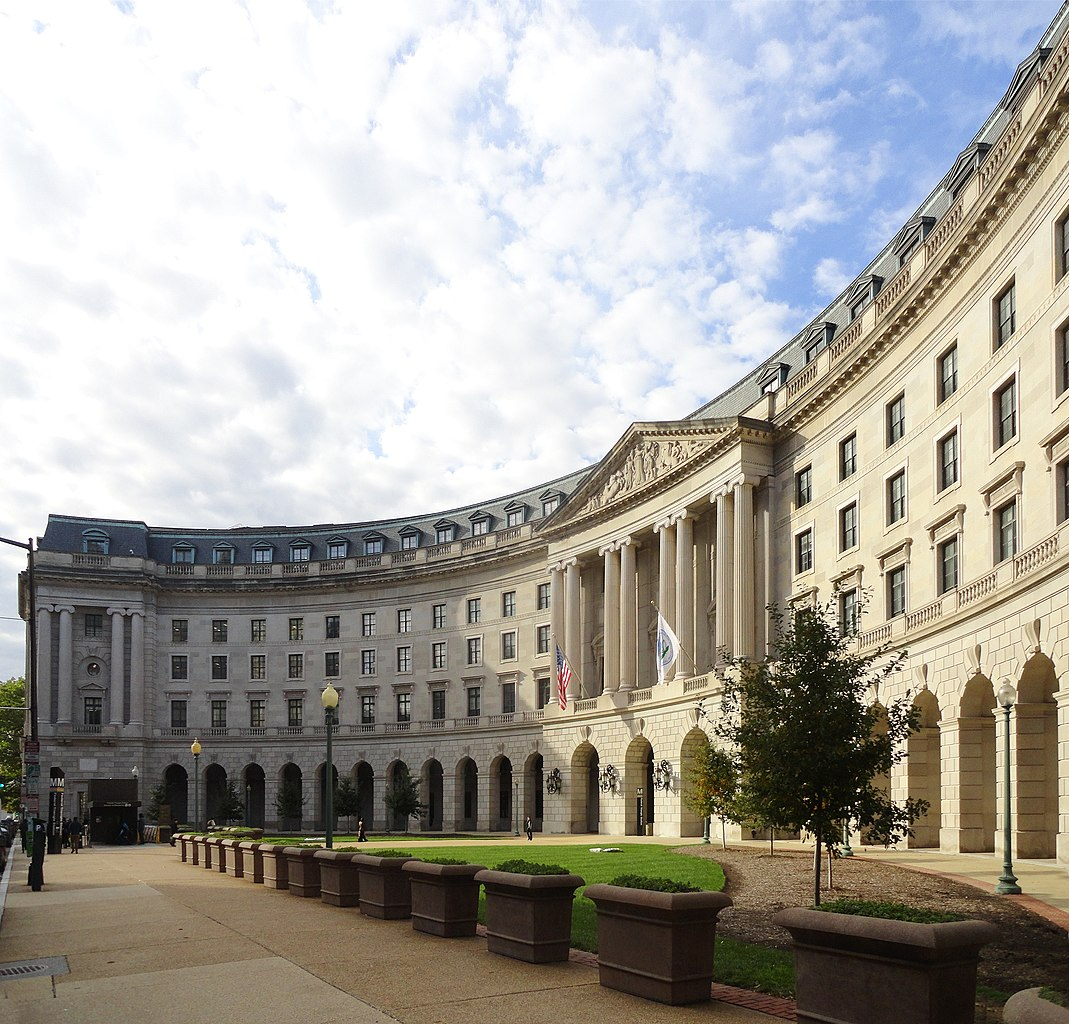
\includegraphics[height=5cm]{figures/us_gov_traditional_1.jpg} }}
    \caption{Left: The Robert C. Weaver Federal Building on 7th Street SW in Washington, D.C., designed in 1965 by Marcel Breuer. It presently serves as the headquarter of the United States Department of Housing and Urban Development. Note that the current occupancy of the building evokes Winston Churchill's famous quote: \textit{"We shape our buildings, thereafter they shape us."} \cite{noauthor_churchill_nodate}. Right: The William Jefferson Clinton Federal Building on Pennsylvania Avenue in Washington, D.C., designed in 1934 by William Adams Delano and Chester Holmes Aldrich. It presently serves as the headquarters of the Environmental Protection Agency. Images of this nature formed the core part of the 2020 American poll on architectural preferences \cite{noauthor_americans_2020}. All image pairs presented showed images of similar shape and purpose, thereby accounting for major non-aesthetic considerations. \newline Image sources (left to right): \cite{highsmith_robert_2012}\cite{wikimedia_commons_user_moreau1_epa_2018}}
    \label{fig:federal_buildings}
\end{figure}

\clearpage
\begin{multicols}{2}

The concept of beauty in architecture has sparked ceaseless and unresolved discussions and controversies. This mirrors equivalent discussions by philosophers from Plato (Symposium, ca. 370BC \cite{plato_symposium_1795}) to David Hume (Four Dissertations: On the Standard of Taste, 1757 \cite{hume_iv_1757}). To Plato, beauty was far from subjective - thereby a beautiful building would be one that has order, symmetry, proportion, harmony, and purpose, and that reveals the essence and goodness of the Form of Beauty. To Hume, beauty was not an inherent property of an object but purely subjective - a beautiful building would be one that pleases the taste of a true judge, who has a refined and cultivated ability to perceive and appreciate beauty, based on experience, comparison, and reflection (an "Architect").

Neuroscience and psychology have only recently been able to contribute significantly to this debate. Research interest in the concept of beauty in architecture has increased exponentially over the past 20 years. Following a preliminary literature review, we found that the research, so far, has been conclusive:

% \footnote{The Elsevier Scopus scientific publication database clearly shows this trend. A search query for publications exploring the relationship between beauty in architecture in the context of psychology and neurology shows an exponential increase: \texttt{TITLE-ABS-KEY((architecture AND beauty) AND (psycho* OR neuro*))}} 

\textit{"Built spaces that facilitate a feeling of awe may have far-reaching positive effects on health and prosocial behaviors."} \newline - Negami et al. (2023) \cite{negami_how_2023}

\textit{"(Fractals) needs to reintegrate with biophilic and traditional architecture in urban design for their proven positive effects on health and well-being. Such benefits include striking reductions in observers’ stress and mental fatigue."} \newline - Brielmann et al. (2022) \cite{brielmann_what_2022}.

\textit{"Built environments that integrate representations of the natural world into façades and interiors benefit occupant psycho-physiological wellbeing and behavior. However, the biophilic quality of buildings does not depend exclusively on “green”, but also upon “organized complexity” in their structure."} - Berto et al. (2022) \cite{berto_biophilic_2022}

\textit{"(...) greenery and other natural features in the built environment may improve mood (...) and accelerate recovery from stress and surgery.} \newline - Coburn et al. (2017) \cite{coburn_buildings_2017}

Unaffected by the intellectual debate on the exact ontological nature of beauty, large-scale scientific studies have advanced our understanding of the aesthetic features which endow the built environment with healing qualities. Initial results point to natural forms, which for millennia have inspired the design of man-made structures, and the many geometric forms that take inspiration from them. Absent in modernist designs, they permeate the facades of many historical buildings in Europe and beyond. Lavdas and Salingaros have gone furthest, proposing a methodology to determine what they blodly claim to be an \textit{"objective measure for beauty"}, as shown in \cref{fig:heatmap}. t Could it be that \textit{"the architect has no clothes"} \cite{mehaffy_architect_2011}?

\end{multicols}

\begin{figure}[H]
    \centering
    \subfloat{{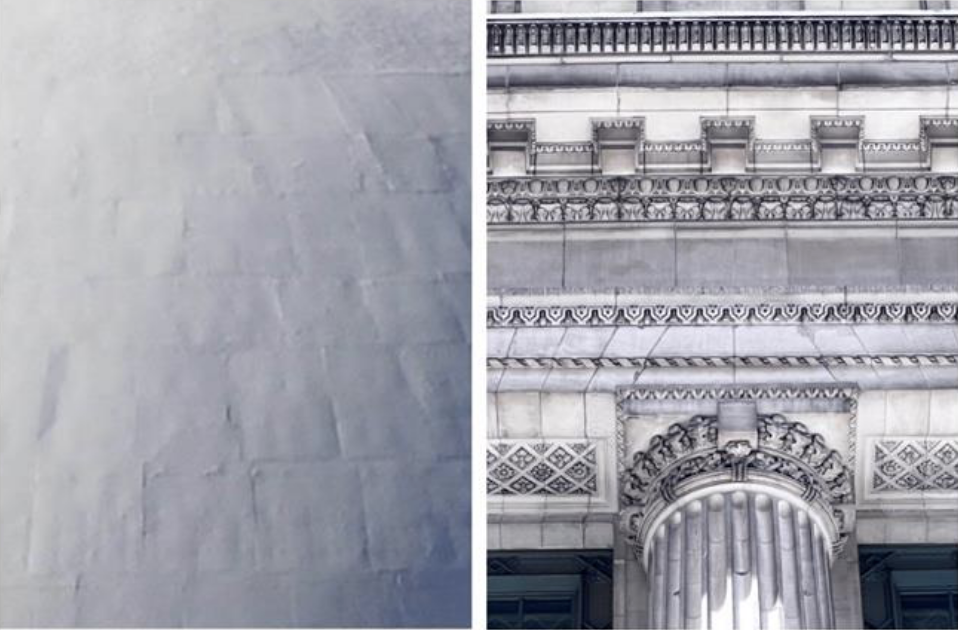
\includegraphics[height=4.75cm]{figures/beautyscale_image.png} }} \hspace{2.5mm}
    \subfloat{{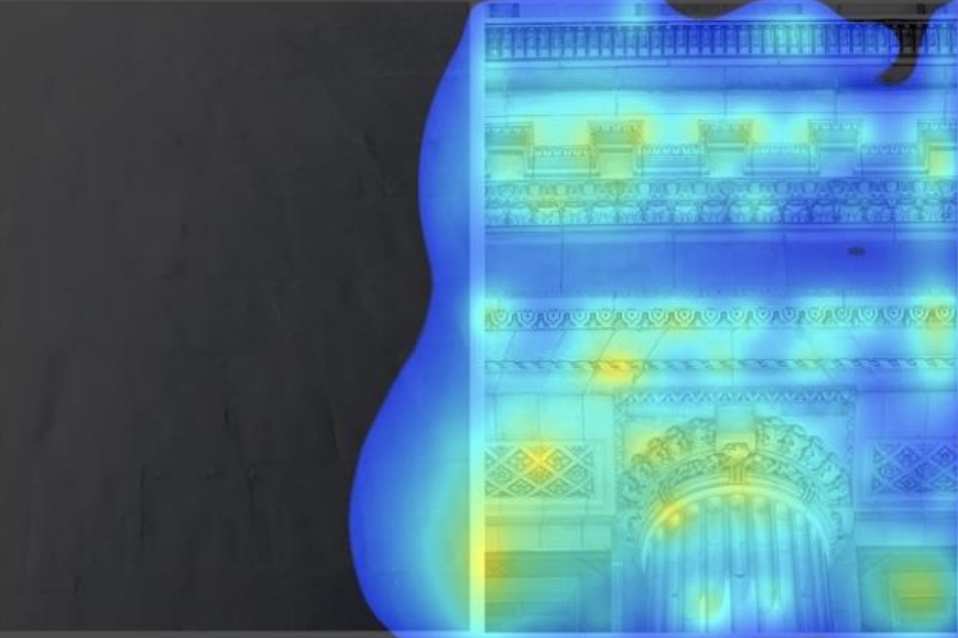
\includegraphics[height=4.75cm]{figures/beautyscale_heatmap.png} }}
    \caption{Left: Two designs for a building facade. Right: A heatmap reveals the degree to which the two different facade designs capture the attention of study participants. The heatmap was generated from eye-tracking data. As expected, the feature-rich pillar capital and lower-side cornice of the right facade retains visual attention to a much higher degree. Source:Figure 6 from Lavdas' and Salingaros' seminal publication \textit{"Architectural Beauty: Developing a Measurable and Objective Scale"} \cite{lavdas_architectural_2022}}
    \label{fig:heatmap}
\end{figure}

\clearpage
\section{The Age of Democracy}
\label{sec:democracy}

\begin{multicols}{2}

While the role of art in a free society remains a topic of philosophical debate, contemporary scholars agree that the role of art in democracy can be non-exhaustively defined as \textit{a mode of participation and action that engages the public in dialogue and debate, and that inspires social change and transformation}. Art thereby can be seen not only as the highest form of self-expression but also as a vital element of the democratic process.

Architecture, unlike some of the fine arts, generally serves an immediate purpose beyond that of aesthetic or intellectual expression. In this way it can perhaps most graciously be described as adding to- and expanding on the functionality which civil engineers involved in any construction project aim to provide. This makes the designs of architects ubiquitous. As a result of this omnipresence in public space, it has been recognized as being

\textit{"(...) the most overweening of the arts, and the one that least lets us alone. A gallery we can't walk out of, a book we can't close, an art we can't even turn our back on because it is there facing us on the other side of the street as well (...)} - British poet Blake Morrison in "Lords of Glass, Steel and Concrete" \cite{morrison_lords_1982}

Switzerland is consistently ranked as of the most democratic nations globally \cite{noauthor_economist_2023} with the principles of subsidiarity and direct democracy forming a vital part of Swiss national identity. At the same time, home ownership remains elusive for the majority of the population, having stagnated at around 40\% over the past decades \cite{noauthor_home_2022}. Aesthetic decisions are therefore further removed from the population. The majority of propoerties that is rented out, is owned by large corporations \cite{noauthor_wem_nodate}.

We have already shown in \cref{sec:ugliness} that a number of polls and scientific studies have replicated the same finding: A cross-cultural rejection of the aesthetic language of modernism and internationalism. In fact, a sentiment that was brought to prominence by Swiss architect Le Corbusier is that of calling for a re-education of the public such that they might come to appreciate their brutalist/modernist designs. The modern version of this is perhaps best exemplified by the reaction of Corbu's compatriot Rudolf Guyer, who in 1955 designed a high-rise residential apartment in southern Zurich. When the building was voted "Switzerland's ugiest building" in 2018 by readers of the daily newspaper \textit{20 Minuten}, he declared:

\textit{"Dass Laien das Gebäude hässlich finden, ist mir egal. Hauptsache, den anderen Architekten gefällt es."} (en.: I don't care that laypeople find the building ugly. The main thing is that the other architects like it) 

So what does it say about the relationship between art and architecture and the public if perhaps the most inescapable form of public art is being rejected by the majority of the population? This questions is multi-facetted, branching into economics, psychology and philosophy.

We mention only one possible solution to this problem: A "revolt against 'ugly' modern architecture" \cite{gersten_scandinavian_2023}

\cref{fig:vienna} and \cref{fig:budaptest} show two diametrically opposed approaches to the replacement of existing building stock in cities that share a similar socio-economic and architectural legacy. 

In fact, we can observe that there is a kind of self-propagating effect: architectural prizes are given out only by architects. There is no 'public vote'. The contempt with which architects have treated the public is by no means covert. 


\end{multicols}

\begin{figure}[ht!]
    \centering
    \subfloat{{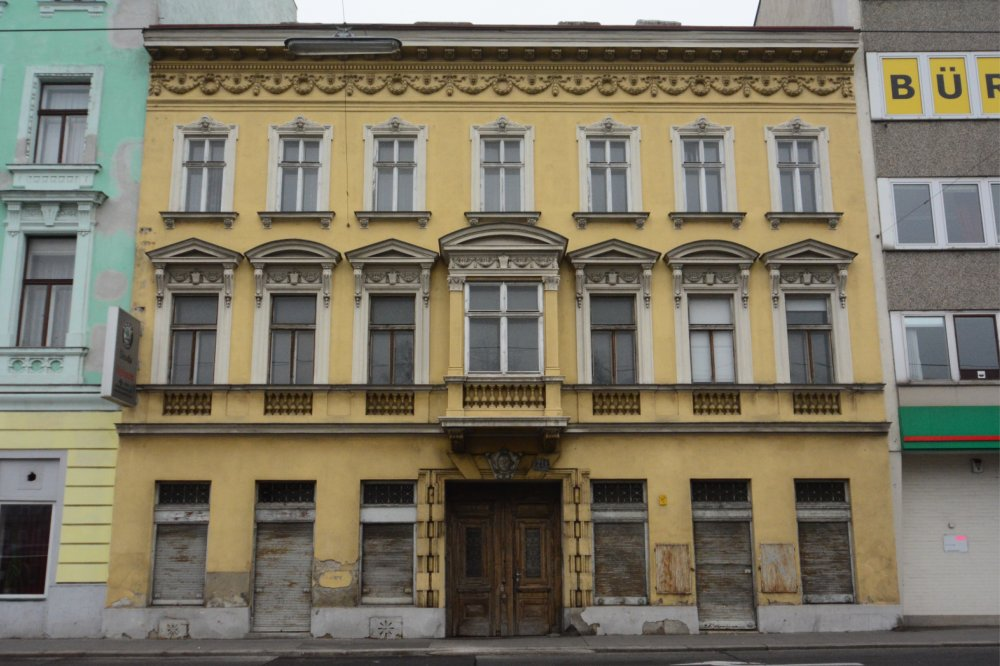
\includegraphics[height=5cm]{figures/vienna_1.jpg} }}
    \subfloat{{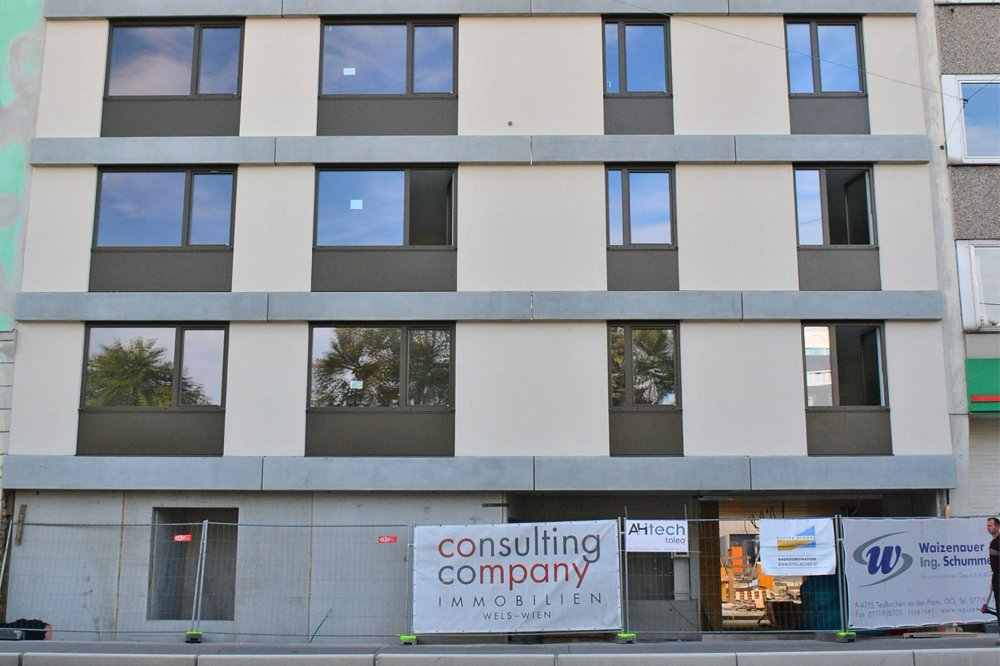
\includegraphics[height=5cm]{figures/vienna_2.jpg} }}
    \caption{Before-and-after: Demolition and reconstruction of a 19th century Gründerzeit style Vienna town house on Schönbrunner Strasse (12th District), as documented by Georg Scherer of the architecture watchblog \texttt{wienschauen.at} \cite{scherer_zerstorung_nodate}. Image sources (left to right): \cite{scherer_schonbrunner_2018}\cite{wikimedia_commons_user_guentherz_wohnhaus_2014}}
    \label{fig:vienna}
\end{figure}

\begin{figure}[ht!]
    \centering
    \subfloat{{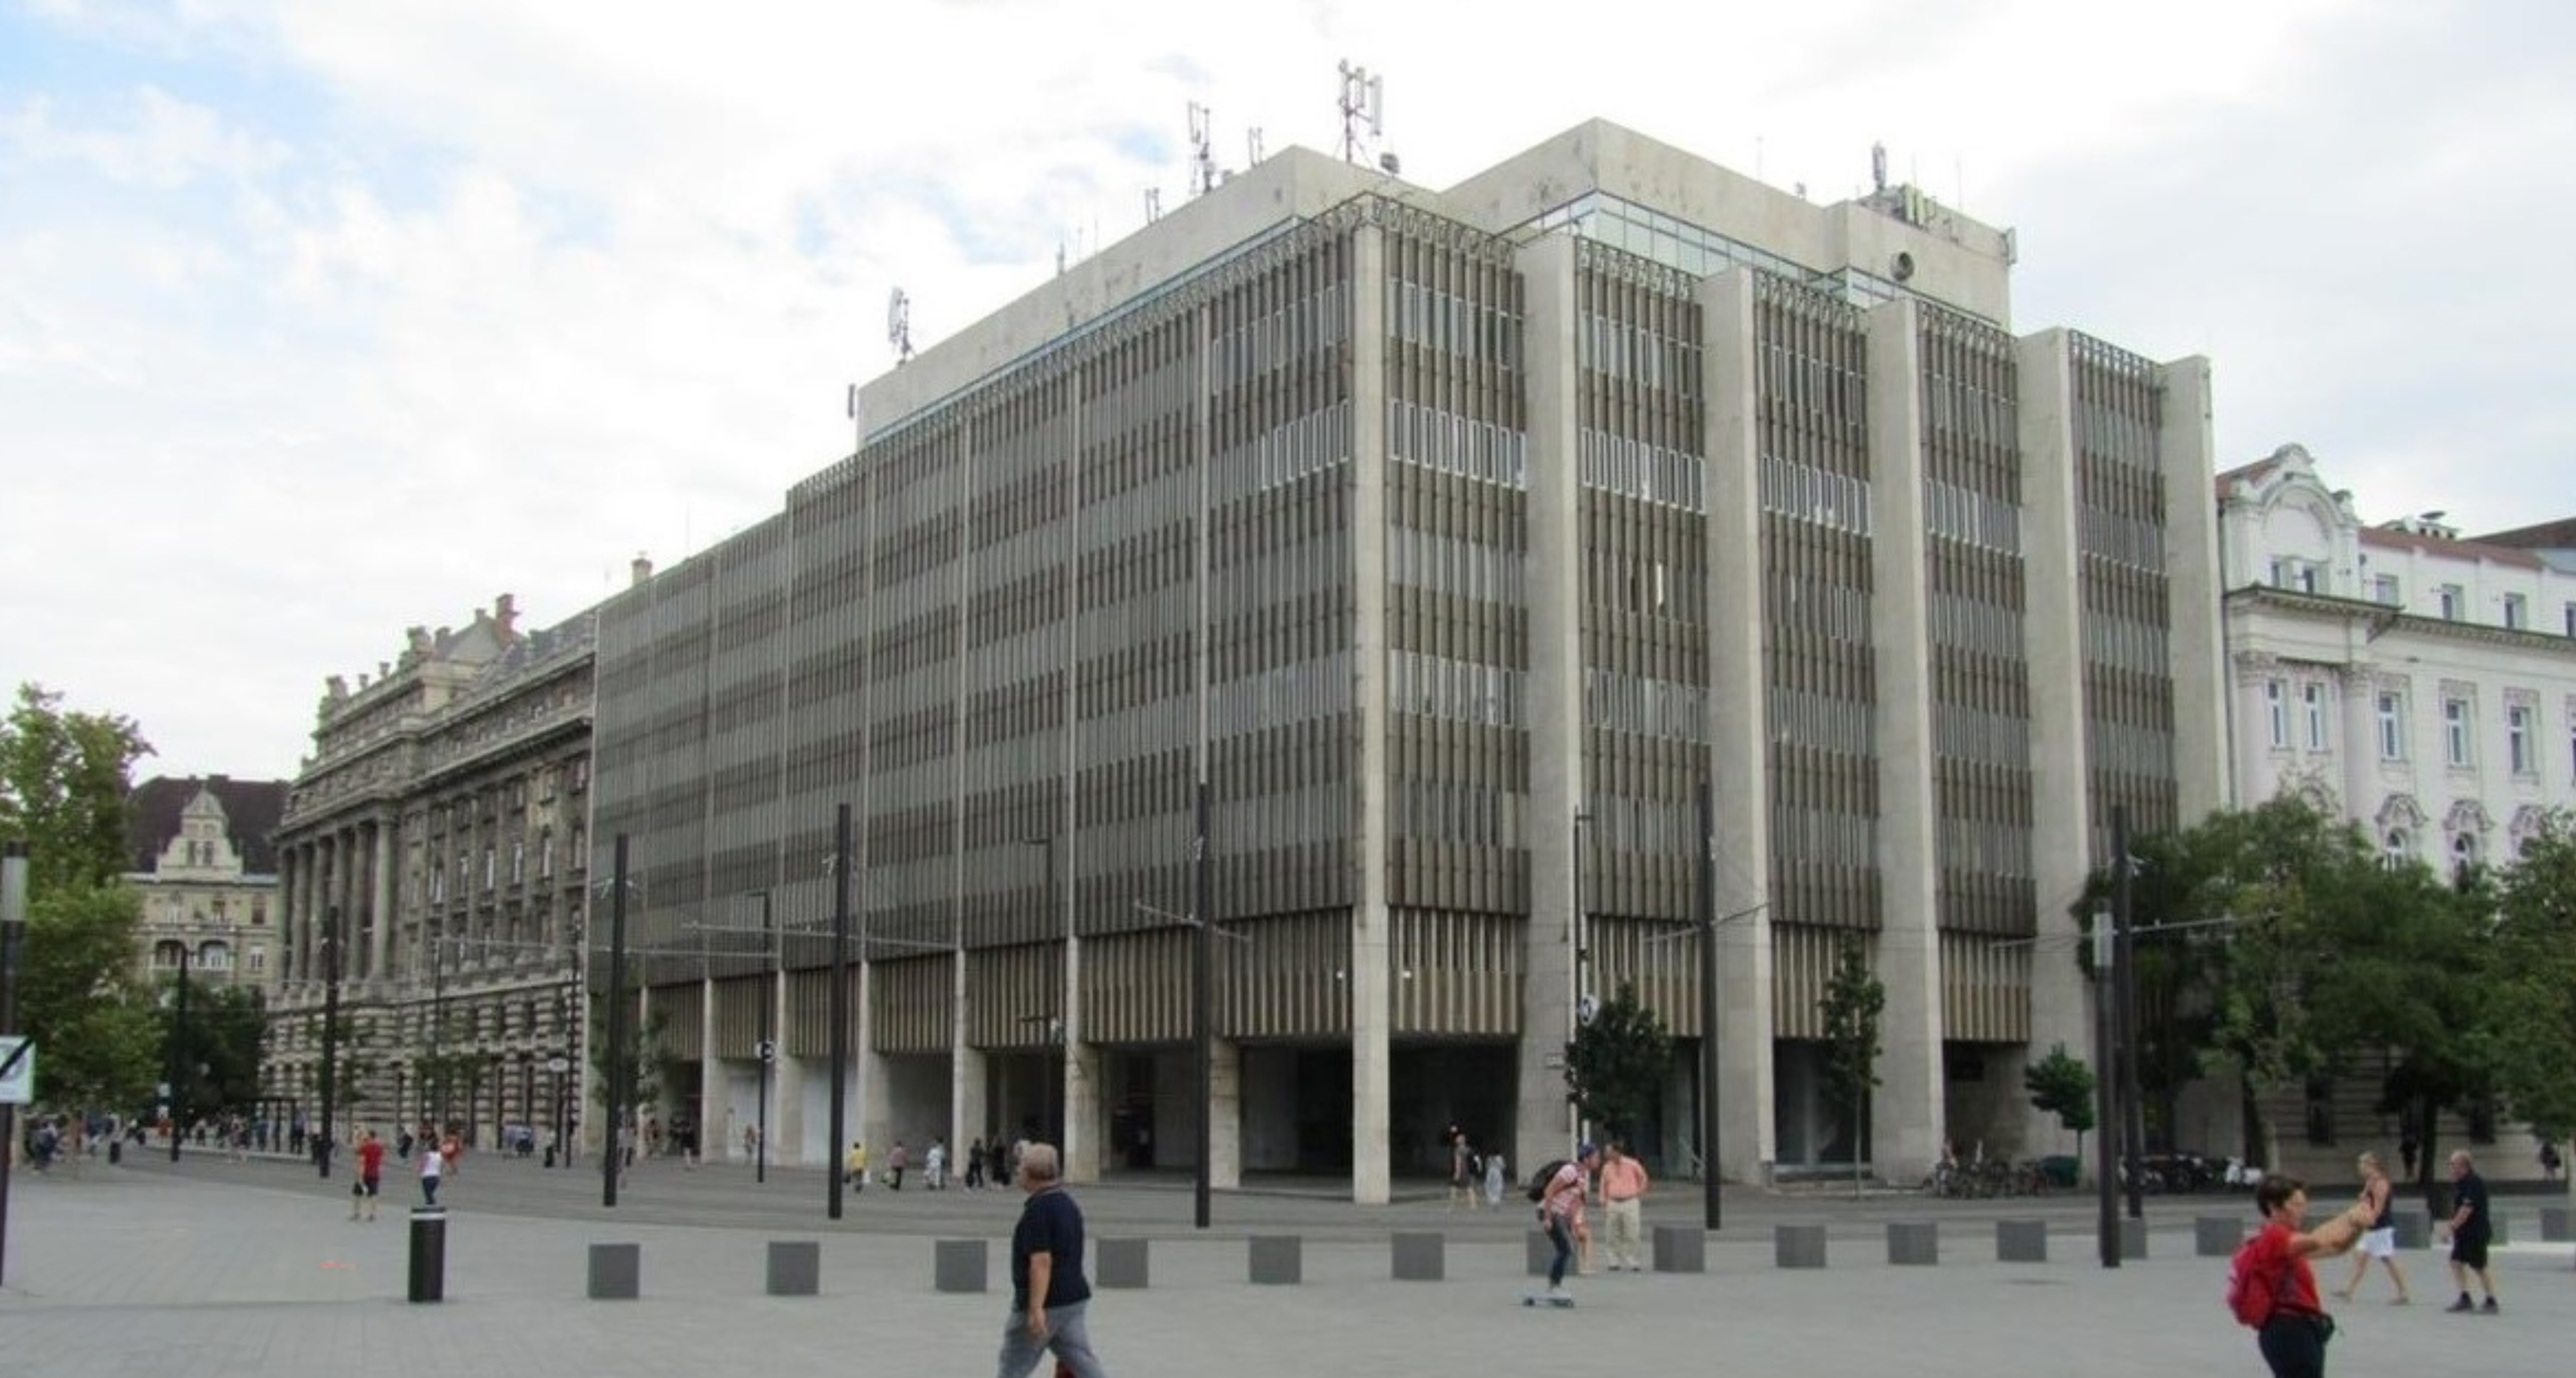
\includegraphics[height=4cm]{figures/hungary_1.jpg} }}
    \subfloat{{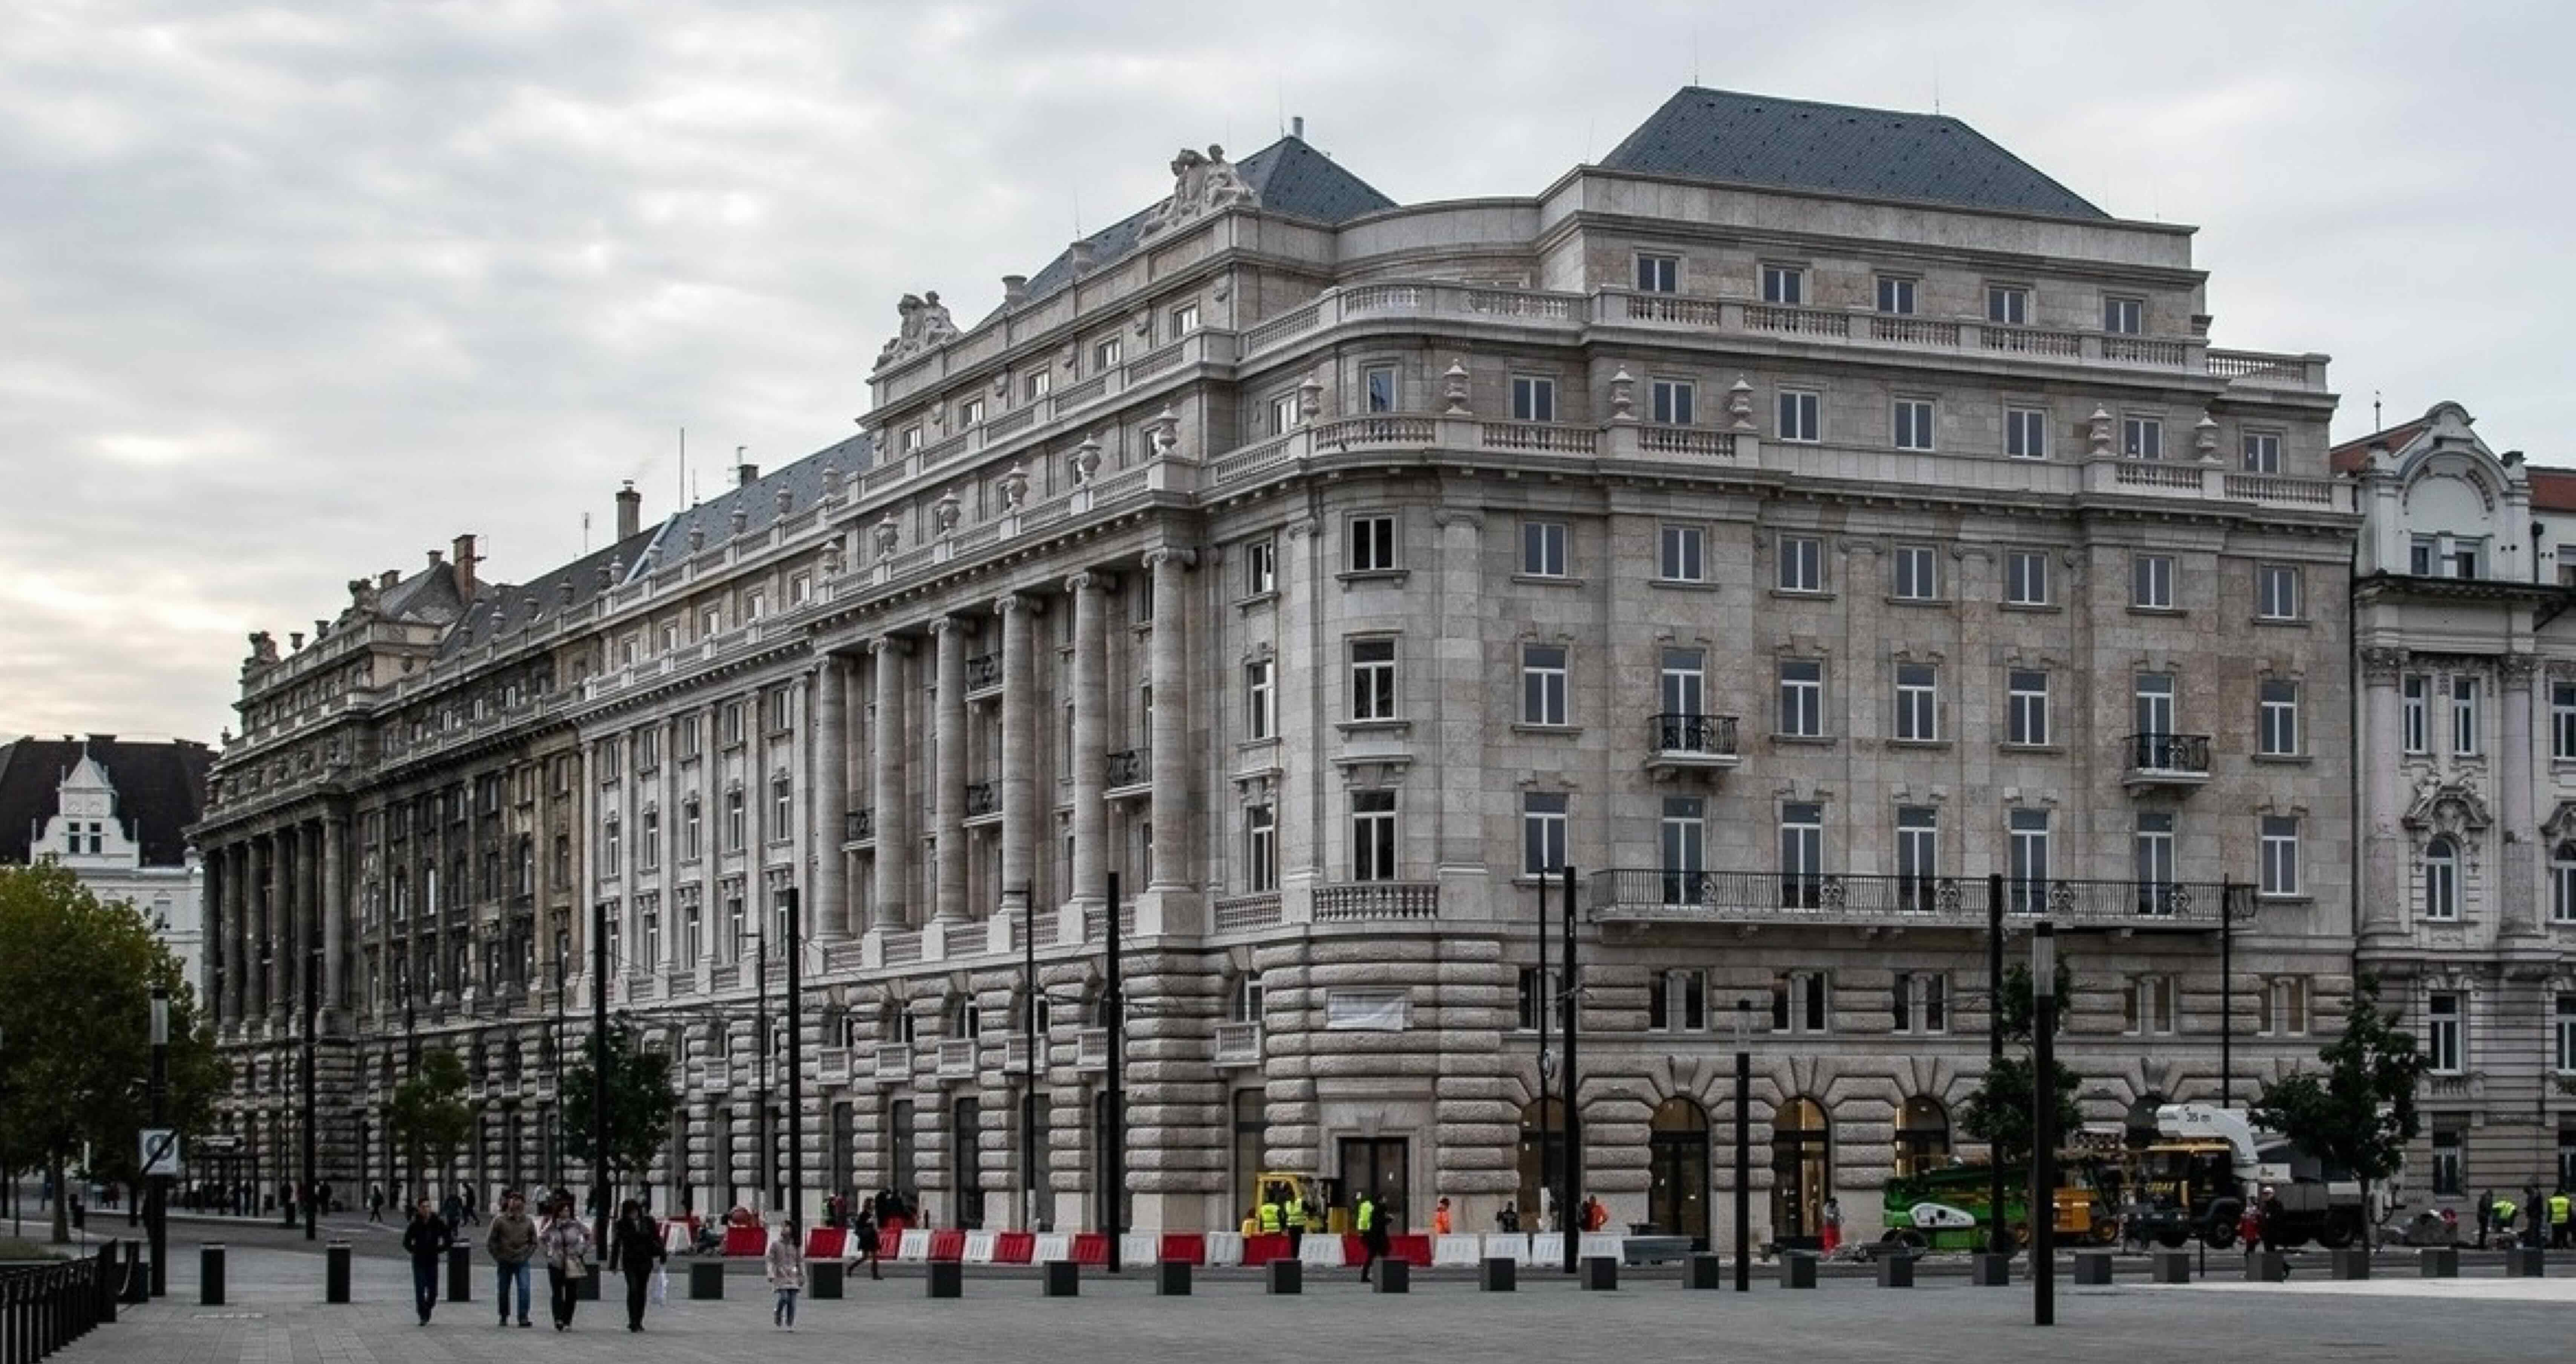
\includegraphics[height=4cm]{figures/hungary_2.jpg} }}
    \caption{Before-and-after: Demolition and reconstruction of a 1970s office building on Kossuth Lajos Square in Budapest, adjacent to the Hungarian Parliament Building, as documented by Michael Diamant of the architecture watchblog \texttt{newtrad.org}. The brutalist style design was intended to replace the unrealized wing of an earlier neo-classical style building. This wing was finally realized according to the original design following the demolition of the 1970s building. Image sources: Adapted from original photographs by Michael Diamant in \cite{natalia_michael_2021} }
    \label{fig:budaptest}
\end{figure}


\begin{comment}

\begin{figure}[ht!]
    \centering
    \subfloat{{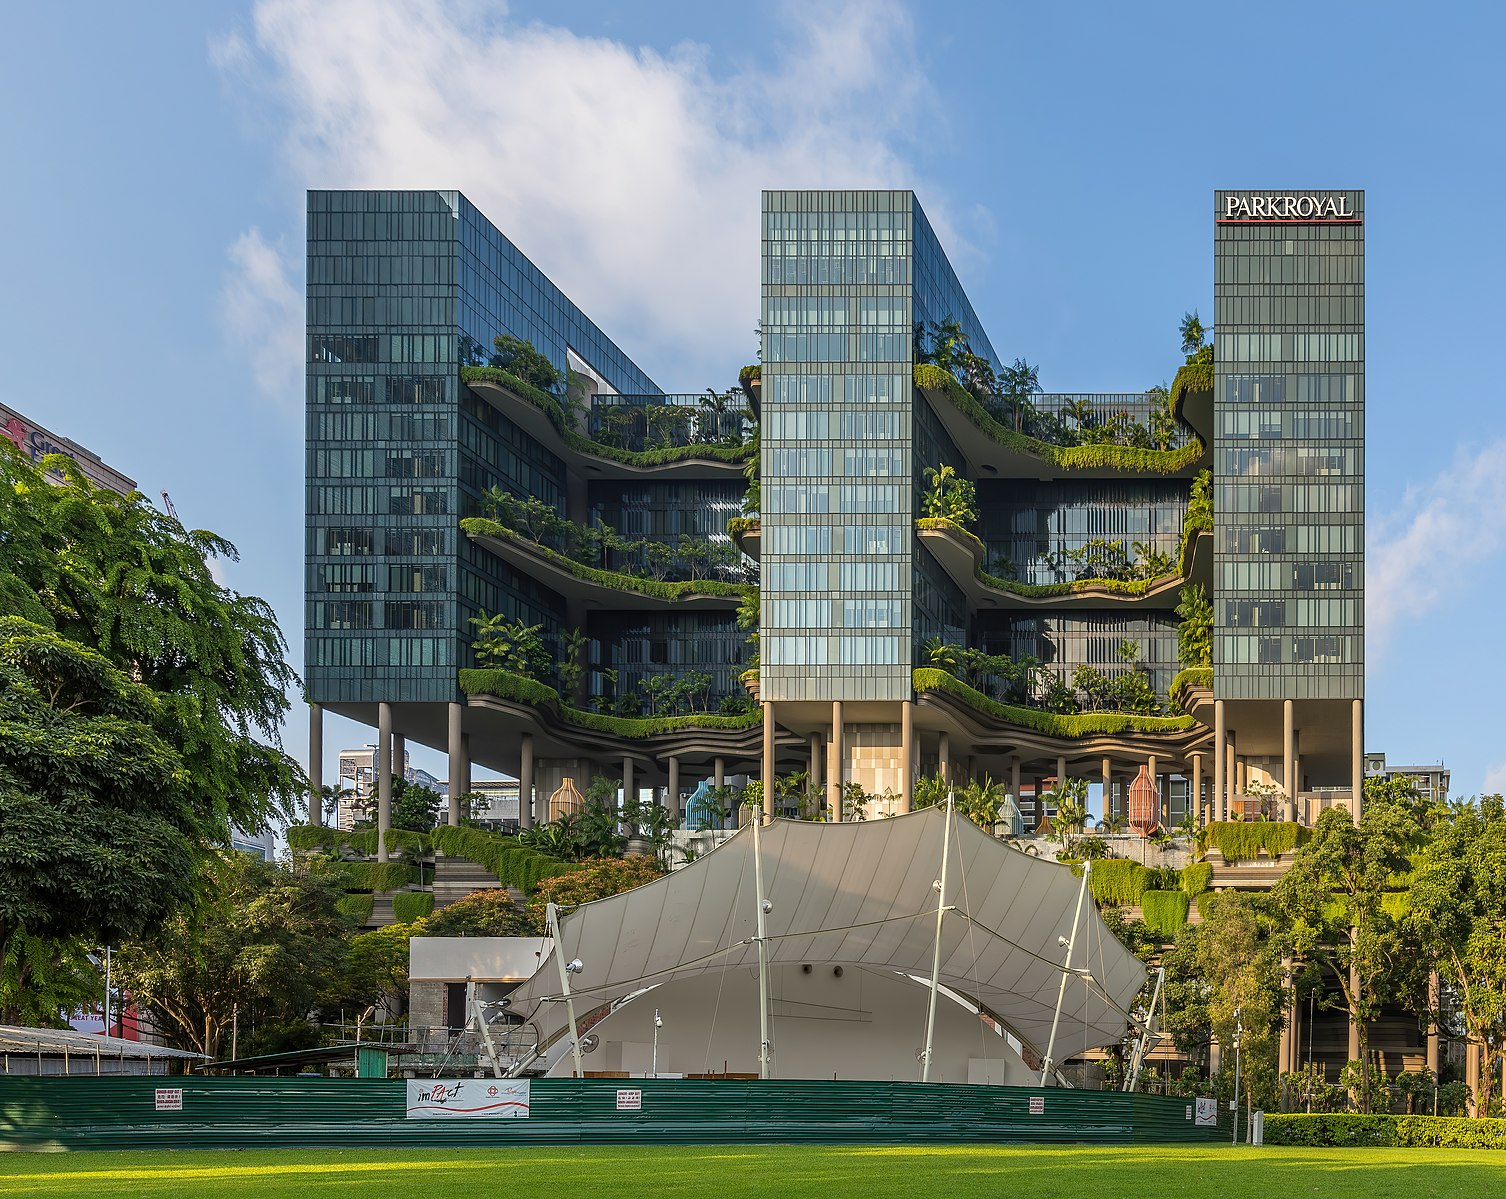
\includegraphics[height=5cm]{figures/parkroyal_1.jpg} }}
    \subfloat{{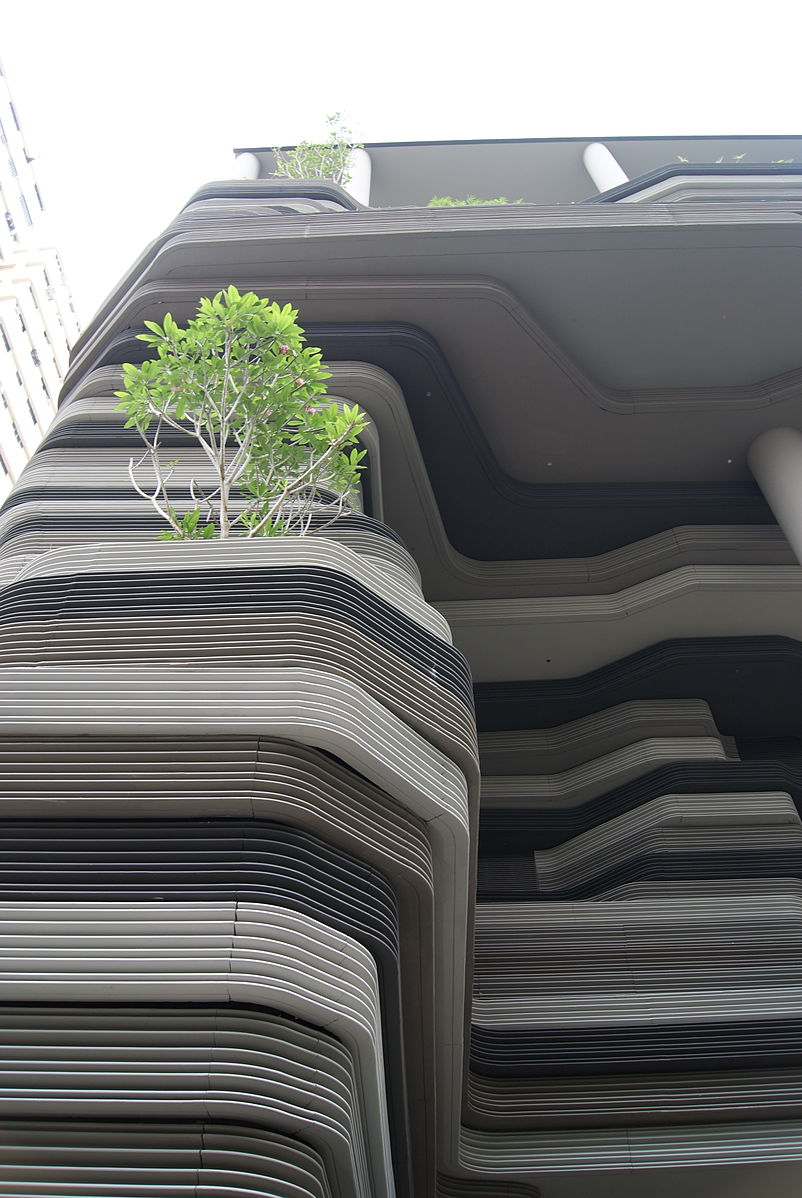
\includegraphics[height=5cm]{figures/parkroyal_2.jpg} }}
    \caption{The \textit{Parkroyal Collection Pickering} luxury hotel on Upper Pickering Street in Singapore, designed by members of the firm WOHA in 2013. Often described as a "garden in a hotel" \cite{hill_take_2021}, the building features multiple terrace gardens utilizing rainwater collection as part of its water management system. Left: Frontal view of the hotel from Hong Lim Park. Right: Detail of the concrete facade with solitary vegetation. Image sources (left to right): \cite{morin_hotel_2018}\cite{smu_constitutional_and_administrative_law_wikipedia_project_parkroyal_2013}}
    \label{fig:parkroyal}
\end{figure}

\end{comment}

\clearpage
\section{A New Age of Biophilic Design}
\label{sec:biophilic}

\begin{multicols}{2}

As we demonstrated with multiple excerpts from recent publications, "biophilic design" in architecture has been frequently highlighted as having positive effects on the aesthetic experience, and by extension the overall wellbeing, of study participants. Biophilic design is a novel term describing an age-old aspiration in architecture: to increase the connection between people and nature in the built environment. It is based on the idea that humans have an innate tendency to seek and appreciate natural elements, such as plants, animals, water, light, and shapes. Biophilic design uses \textit{direct nature, indirect nature, and space and place conditions} to create environments that are beneficial for human health, well-being, and sustainability \cite{kellert_practice_2015}. One example of the indirect use of nature is provided by the lavish floral ornamentation in Jugendstil (en.: Art Noveau) design. Perhaps the most well-known fully nature-inspired structure was the monumental arch of the 1900 Paris expo, as depicted in \cref{fig:porte_binet}, inspired by contemporary artistic depictions of microscopic life-forms shown in \cref{fig:kunstformen}.
    
\end{multicols}
\vspace{-5mm}

\begin{figure}[ht!]
    \centering
    \subfloat{{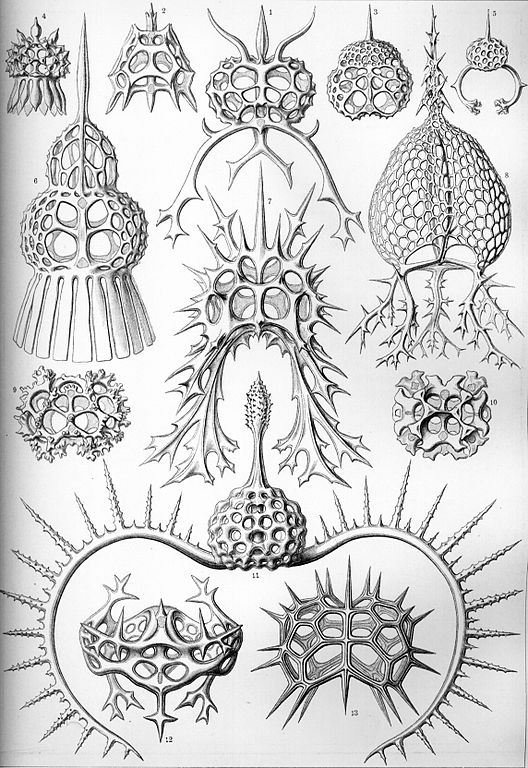
\includegraphics[height=5cm]{figures/Spyroidea.jpg} }}
    \subfloat{{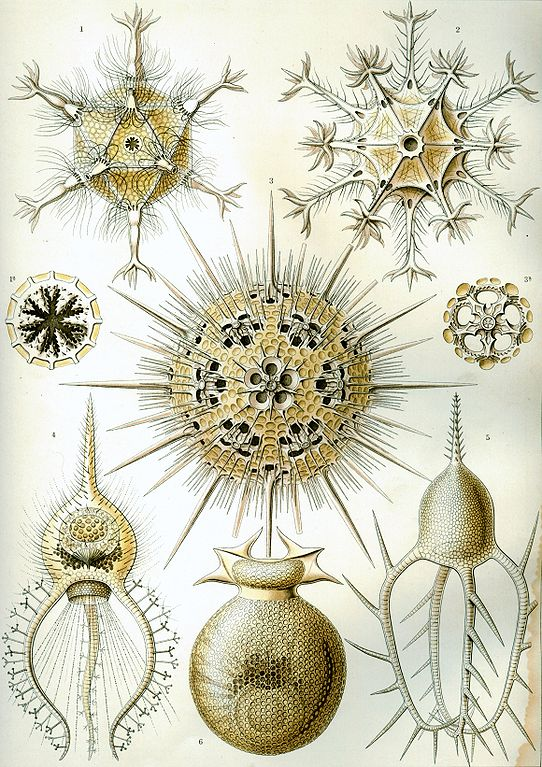
\includegraphics[height=5cm]{figures/Phaeodaria.jpg} }}
    \subfloat{{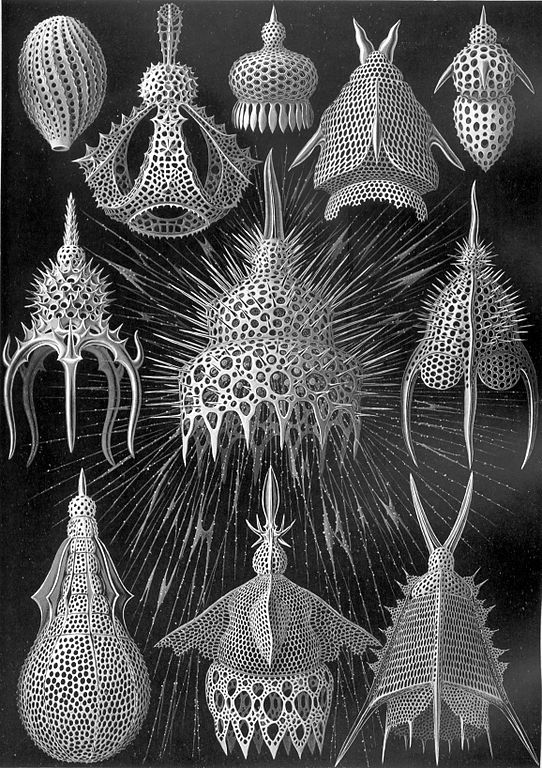
\includegraphics[height=5cm]{figures/Cyrtoidea.jpg} }}
    \caption{Selection of drawings from Ernst Haeckel's \textit{Kunstformen der Natur} (en.: "Art Forms in Nature") \cite{haeckel_kunstformen_2012}. According to architect Rene Binet, these drawings served as direct inspiration for his monumental arch \cite[Sec. "Haeckel und der Jugendstil"]{willmann_haeckel_2019}, which is depicted in \cref{fig:porte_binet}. \newline Image sources (left to right): Spyroidea \cite{haeckel_kunstformen_1904}, Phaeodaria \cite{haeckel_kunstformen_1904} and Cyrtoidea \cite{haeckel_kunstformen_1904-2}.}
    \label{fig:kunstformen}
\end{figure}\vspace{-5mm}

\begin{figure}[ht!]
    \centering
    \subfloat{{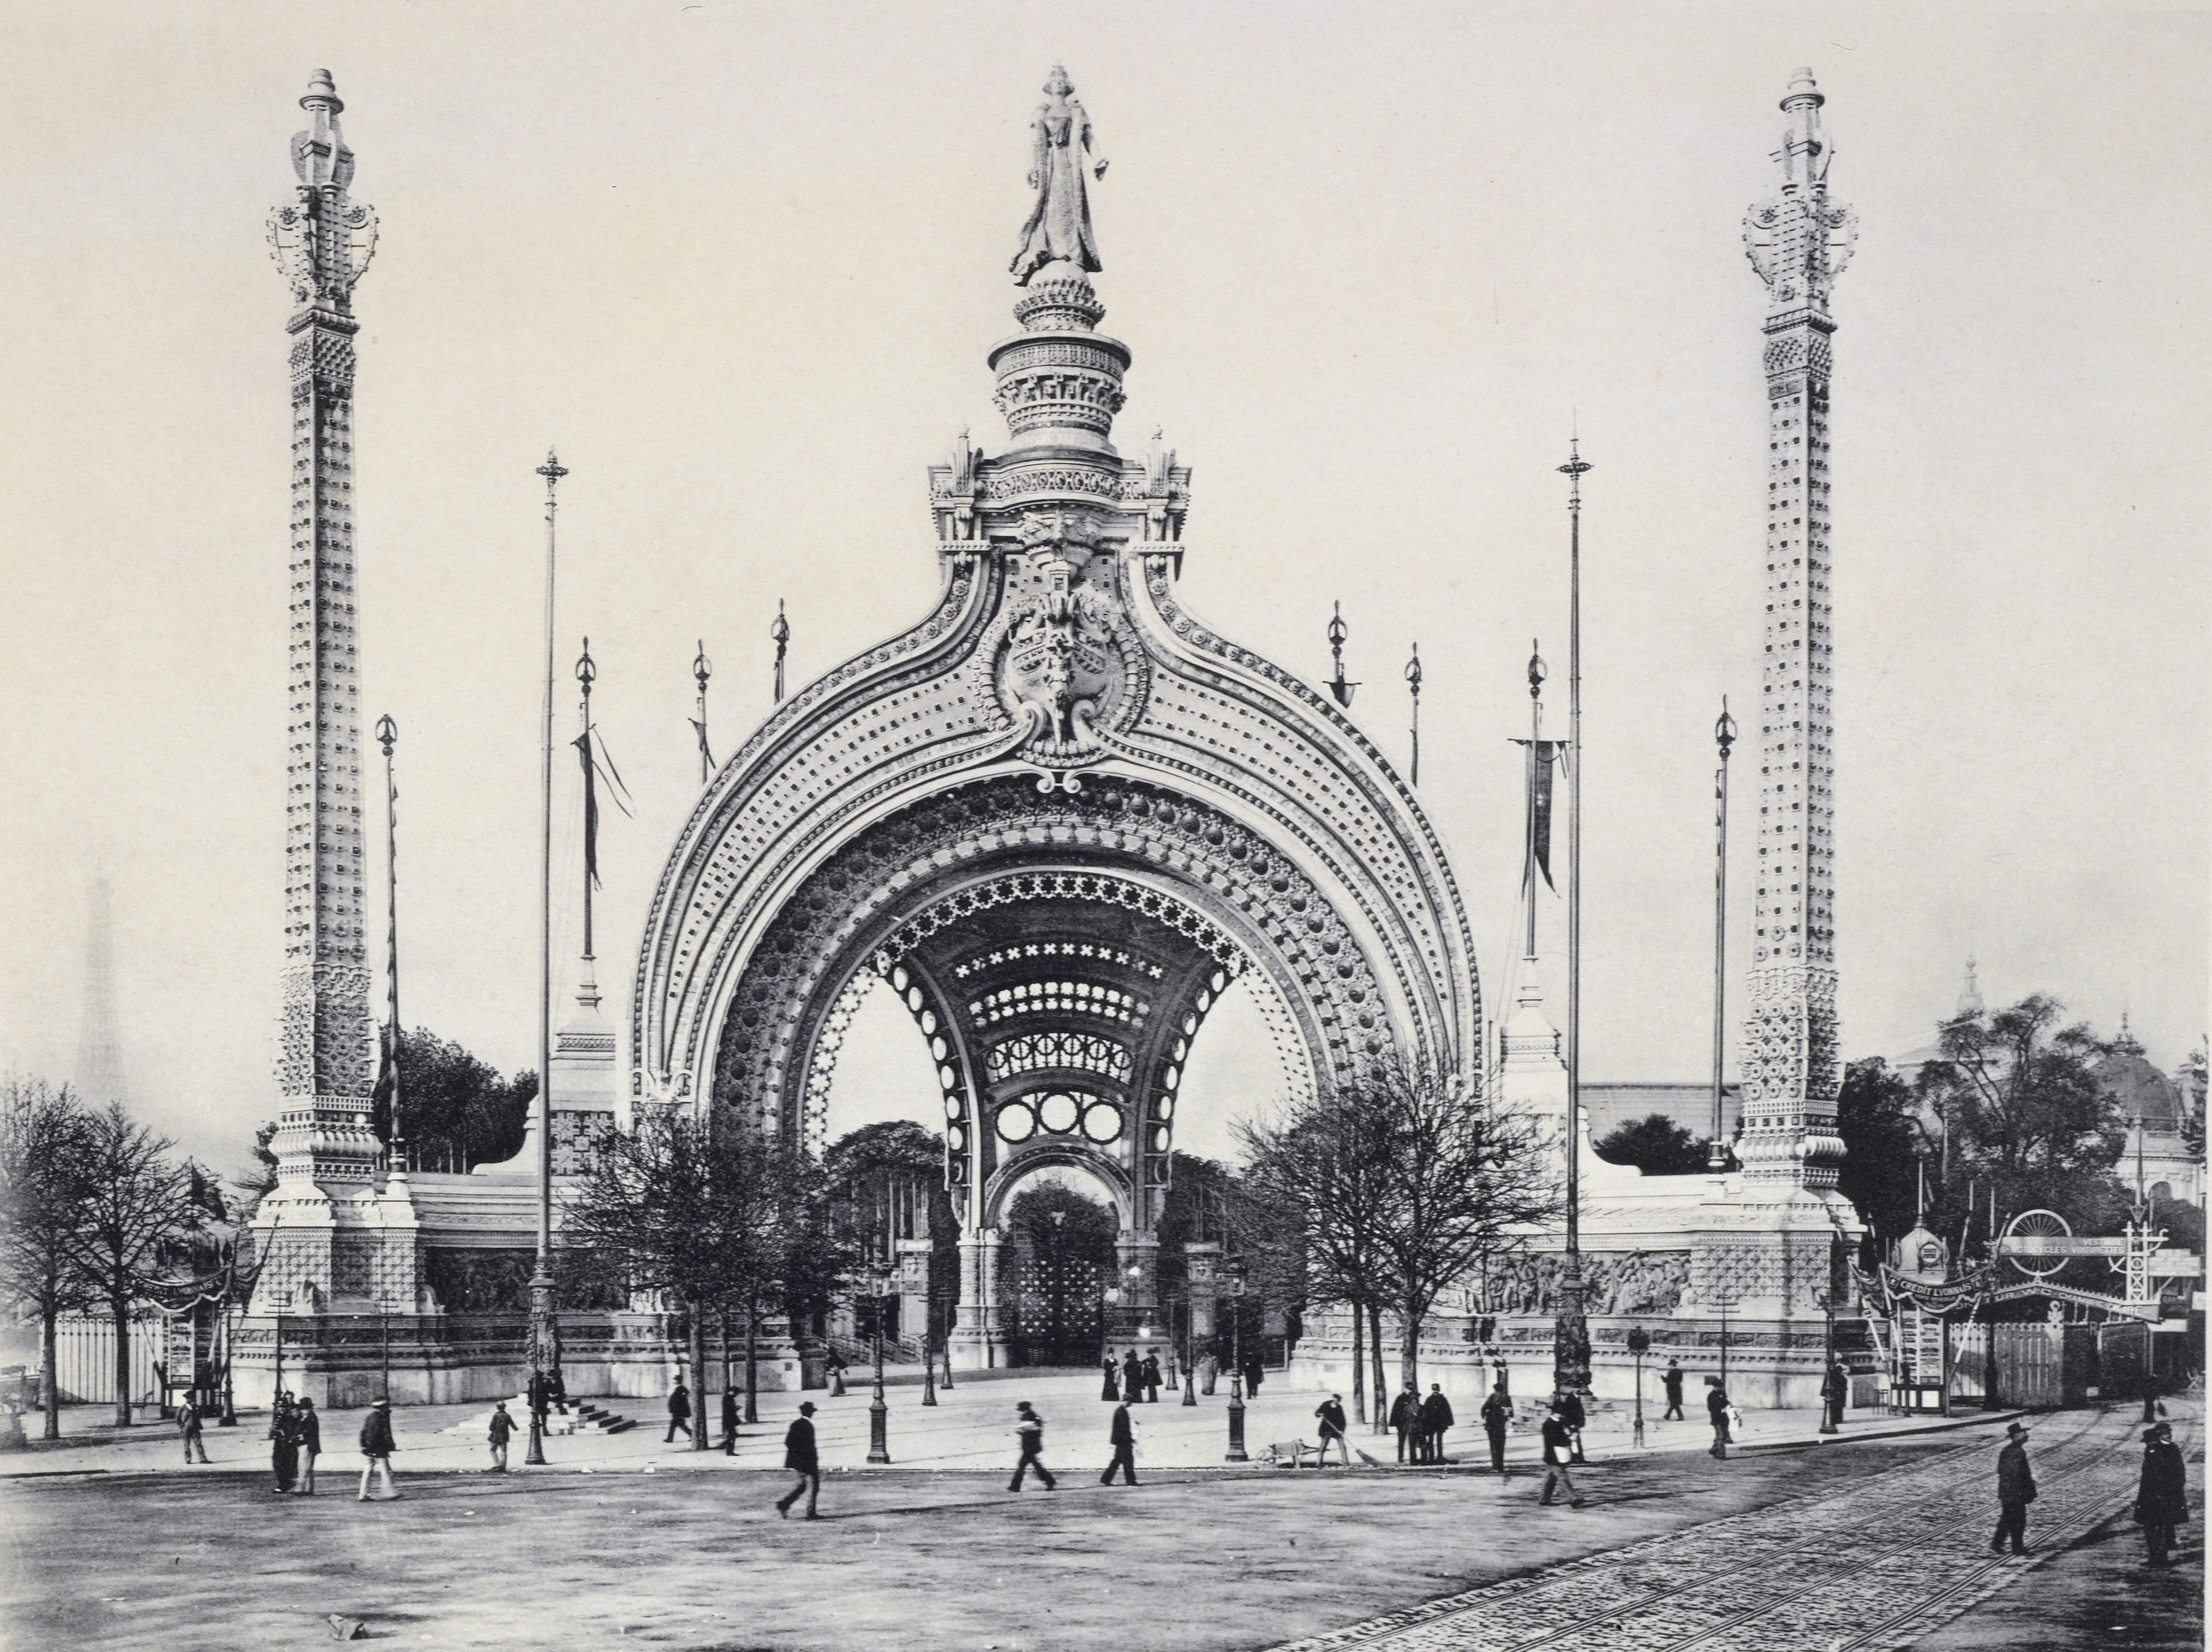
\includegraphics[height=5cm]{figures/porte_photograph.jpg} }}
    \subfloat{{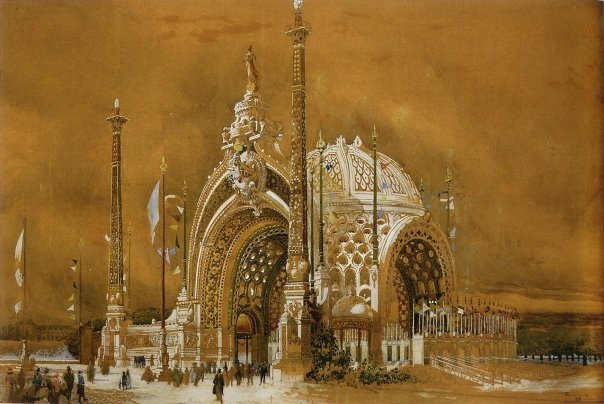
\includegraphics[height=5cm]{figures/porte_watercolor.jpg} }}
    \caption{Two renderings of the \textit{Porte Binet}, a monumental entrance at the site of the 1900 Paris Exhibition, designed by Rene Binet. The structure was composed of a metallic network with embedded coloured glass elements covering over 3000 electric lamps. \newline Image sources (left to right): \cite{louis_porte_1900}, \cite{binet_projet_1898}.}
    \label{fig:porte_binet}
\end{figure}

\clearpage

\begin{multicols}{2}

However, biophilic design can transcend the aesthetic dimension. While nature-inspired functional aspects of construction are often described under the term bio-mimicry, the difference is only semantic. \cref{fig:ventilation} shows what is perhaps the most famous example of functional bio-mimicry in the built environment. 

This ties back in with the sustainability question
while aesthetics can do beautiful buildings
function can do efficiency buildings
perhaps even recyclable buildings

The academic interest in biophilic design has been growing exponentially since 2012, some of which can likely be attributed to the term itself being "in fashion" \footnote{Compare the results of the Elsevier Scopus publication index for the search: \texttt{TITLE-ABS-KEY(biophilic AND design)}}. But will biophilic design emerge as a major new force, a new \textit{Strömung} (en.: architectural tendency), healing wounds that exposed concrete and steel have torn in the fabric of European cities? Will the use of natural materials be able to reduce the environmental burdens of the construction sector, or will architects simply adorn their designs with the odd tree here-and-there to make sure their designs don't look completely out of time? Will ornaments, inspired by forms of nature, once again bloom on the facades - or will real living plants grow on walls, balconies and terraces? Will new developments in neuroscience and psychology be able to help us design better, more beautiful buildings?

It is in this context that we propose a schedule to host a Summer Academy. We believe this will be more than just interesting discussions. We will provide participants with the tools to think critically, to assess and to better understand. \newline - MPW, PS, MCB


\end{multicols}

\begin{figure}[ht!]
    \centering
    \subfloat{{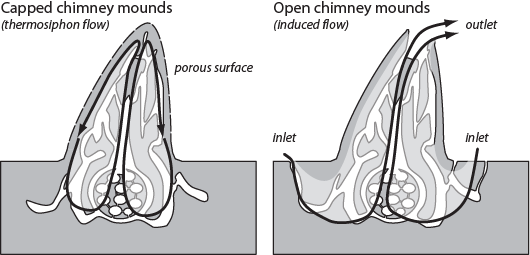
\includegraphics[height=4cm]{figures/termite_crossection.png} }}
    \subfloat{{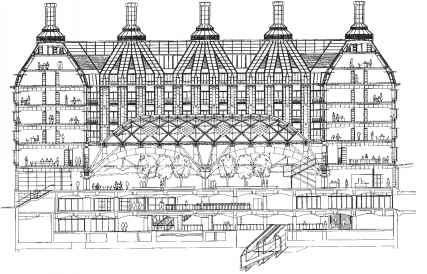
\includegraphics[height=5cm]{figures/portcullis_crossection.jpg} }}
    \caption{Energy-efficient air-flow cooling inspired by the design of termite mounds. Left: Cross-section of the mounds of two different termite species, one with open air vents and one with a porous surface. Right: Cross-section of \textit{Portcullis House} on Bridge Street in London, designed by members of the firm Michael Hopkins and Partners in 1992. The tall chimneys form part of the termite-inspired air circulation system, utilizing the stack effect to create an updraft. \newline Image sources (left to right): \cite{turner_beyond_2008}, \cite{davies_hopkins2_2001}.}
    \label{fig:ventilation}
\end{figure}


\clearpage
\section{Proposed Schedule}
\label{sec:schedule}

\subsection{Day I: History of Architecture}

\begin{NiceTabular}{W{l}{3cm}l}[]
\textit{Primary Instructor} & Samuel Leder \\
\textit{Teaching Assistant} & Philippe Schultheiss \\
\textit{Didactic Format} & Lecture and Discussion Groups
\end{NiceTabular}

\textit{To what degree is architecture political or ideological? How did the political upheavals of the early 20$^{\text{th}}$ century shape decades of buildings design to come? Which are the major trends in architectural design today - and how, if at all, do they interact? Students of engineering or the natural sciences often have only a limited understanding of the politics that shape the academic landscape at firms and academic architecture departments. On this day, the participants will be guided through two millennia of architectural history, with a specific focus on the origins of the modernist movement. It will provide important context for discussions on the following days.}

\href{https://www.linkedin.com/in/samuel-leder/}{Samuel Leder \ExternalLink} is the program manager of the Urban Management course at the Center for Urban and Real Estate Management at the University of Zurich. Following his studies in architecture at ETH Zurich, he worked in a Basel-based architecture firm. He presently serves as co-president of the association \href{https://www.placemaking-switzerland.ch}{Placemaking Switzerland \ExternalLink}, where he drives the development of  community-based, livable, socially and ecologically sustainable settlement areas and neighborhoods. An alumnus of the Swiss Study Foundation, his discussion with the authors of this document have been instrumental in shaping the proposed framework.

\subsection{DAY II - Sustainability in the Built Environment}

\begin{NiceTabular}{W{l}{3cm}l}[]
\textit{Primary Instructor} & Dr. Martin Röck, Dr. Romain Sacchi and Michael P. Weinold \\
\textit{Teaching Assistant} & Mark C. Ballandies \\
\textit{Didactic Format} & Computer-Based Interactive "Sustainability Lab" Group Work
\end{NiceTabular}

\textit{What is the environmental impact of a concrete-and-steel building? How does it fare against a clay-and brick building with wood beams and hemp insulation? How complex is a full life-cycle analysis of a construction project? Do we need expensive reports prepared by sustainability consultants, or can we a reasonable assessment ourselves? Where in the supply chain do emissions occur - which can we avoid and which will take decades to be fully decarbonized? The participants will learn about the fundamentals of environmental assessment and complete an interactive life-cycle analysis of two case-studies.}

\href{https://www.linkedin.com/in/martinroeck/}{Dr. Martin Röck \ExternalLink} is a research associate at Delft University of Technology (Netherlands), where he has been developing a large-scale database of the embodied carbon in the European building stock.\footnote{Embodied-Carbon-of-European-Buildings-Database (EU-ECB-DB), \href{https://github.com/mroeck/Embodied-Carbon-of-European-Buildings-Database}{\texttt{https://github.com/mroeck/}}} His research is focused on  on improving climate and environmental performance of buildings at scale. He applies life cycle-based assessment methods, building information modelling and data science workflows to inform environmental benchmarking and target setting as well as to identify and promote effective building design strategies for advancing a regenerative development of spatial systems at large. Martin holds a Dual PhD in Architectural Engineering from KU Leuven and Engineering Sciences from TU Graz for which he has been awarded a DOC Fellowship by the Austrian Academy of Sciences.

\href{https://www.linkedin.com/in/romainsacchi/}{Dr. Romain Sacchi \ExternalLink} is a tenured researcher in the Technology Assessment Group at  Paul Scherrer Institute (Switzerland). During his postdoctoral research, he developed a powerful mathematical model for prospective environmental modelling that is now used widely in academia and industry. Before returning to academia, he gathered six years of experience in the environmental impact assessment of the construction sector, where he developed sustainability strategies.

\subsection{DAY III - Measuring Beauty}
\label{subsec:day_3}

\begin{NiceTabular}{W{l}{3cm}l}[]
\textit{Primary Instructor} & Dr. Alexandros A. Lavdas \\
\textit{Teaching Assistant} & Michael P. Weinold \\
\textit{Didactic Format} & Lecture and Discussion Groups
\end{NiceTabular}

\textit{Measure beauty? Quantify the aesthetic experience? What a preposterous idea! On this day, the participants will learn about new neurological discoveries that have deepened our understanding of what we perceive as beautiful in a building. The methods most frequently used in the scientific studies listed in \cref{sec:ugliness} will be elaborated. The participants will have the opportunity to interact with the foremost researchers of neuro-aesthetics, who only recently published their latest findings (cf. \cref{fig:heatmap}). This will provide participants with the methodological understanding required to fully appreciate the field trip planned for the last days of the academy.}

\href{https://www.linkedin.com/in/alexandros-a-lavdas-9b127518/}{Dr. Alexandros A. Lavdas \ExternalLink} is a tenured senior researcher at Eurac Research Institute for Biomedicine in Bolzano (Italy), where an imaging laboratory was set up under his guidance in 2014. He is among the most well-known researchers in neuro-aesthetics, having recently proposed a seminal method for the quantitaive measurement of architectural beauty \cite{lavdas_architectural_2022} (compare also \cref{fig:heatmap}). His research enables cell-level imaging that is fundamental for a better understanding of processes and mechanisms, both with regard to the emergence and development of diseases and the effect of drugs. He was previously with University College London, where he carried out research on cortical development, and later, at the Pasteur Institute in Athens, on injury and repair of the central nervous system.



\subsection{DAY IV - A Return to Nature}

\begin{NiceTabular}{W{l}{3cm}l}[]
\textit{Primary Instructor} & Carlo Battisti et al. \\
\textit{Teaching Assistant} & Michael P. Weinold \\
\textit{Didactic Format} & Lecture and Discussion Groups
\end{NiceTabular}

\textit{How can we learn from nature to improve not only the aesthetics of new buildings, but to affect a broader change toward sustainable construction? Will it be enough to plant trees on concrete and steel high-rises, or is this recent trend nothing but the latest large-scale attempt at green-washing in the construction sector? On this day, the participants will engage with one of the foremost thinkers of biophilic design who just recently completed work on a large international research project on sustainable construction.}

\href{https://www.linkedin.com/in/carlobattisti/}{Carlo Battisti \ExternalLink} is the president of \href{https://www.living-future.eu}{\textit{Living Future Europe} \ExternalLink}, a non-profit organization that promotes biophilic design and regenerative development. He is also the founder and leader of the Biophilic Society, a network of biophilic design lovers and professionals. From 2017-2021, he was working with Eurac Research Institute in Bolzano, Italy as Chair and Project Manager of the EU COST Action 16114 "RESTORE" (REthinking Sustainability TOwards a Regenerative Economy). The aim of this research project was to affect a paradigm shift towards restorative sustainability for new and existing buildings and space design across Europe, through the collaboration of 160+ researchers from 40 European countries. He has a degree in Civil Engineering from the Polytechnic University of Milan and about twenty years of experience in construction companies.

\subsection{DAY V - Bringing it all together...}

The schedule for this day will be determined as soon as the majority of the proposed speakers have confirmed their attendance. It would be desirable to combine the ideas developed during the past days in preparation for the field trip scheduled for days VI-VII.

\clearpage
\subsection{DAYS VI-VII - Field Work}

\begin{NiceTabular}{W{l}{3cm}l}[]
\textit{Primary Instructor} & Dr. Alexandros A. Lavdas and Aladar Tepelea \\
\textit{Teaching Assistant} & Michael P. Weinold, Philippe Schultheiss, Mark C. Ballandies \\
\textit{Didactic Format} & Field-Trip with interactive Experiment and Data Analysis
\end{NiceTabular}

\textit{Milan is a city that harmonizes diverse architectural expressions and epochs, from the traditional to the contemporary, from the classical to the innovative. It is the perfect destination for the academy participants to explore the themes that were explored in the lectures and interactive sessions during the first part of the academy. With the help of mobile eye-tracking equipment, we will be able to determine in real time what effects different architectural styles of the build environments can have on our overall well-being and our visual attention. In Milan, the participants will be able to appreciate the splendor and refinement of Gothic cathedrals, Renaissance churches, and Baroque palaces, as well as the "practicality" of modernist skyscrapers, brutalist housing complexes, and newly erected biophilic towers, bursting with greenery. }

For the vita of Dr. Alexandros A. Lavdas, compare \cref{subsec:day_3}.

\href{https://www.linkedin.com/in/aladar-tepelea/}{Aladar Tepelea \ExternalLink} is an Austrian entrepreneur who manages two information technology startups. He has a background in business from Vienna University of Economics as well as extensive work experience with the foremost financial institutions in the United States and in Europe. His company \href{https://www.mindset-technologies.at}{\textit{Mindset Technologies} \ExternalLink} has developed eye-tracking software that can be used to "predict attention" in a number of different environments. The equipment is highly mobile and has already been used to understand where airline pilots focus their attention in the cockpit. With slight modifications, it can be used to re-create the experiments of Dr. Lavdas in a field experiment. 

\begin{figure}
    \centering
    \subfloat{{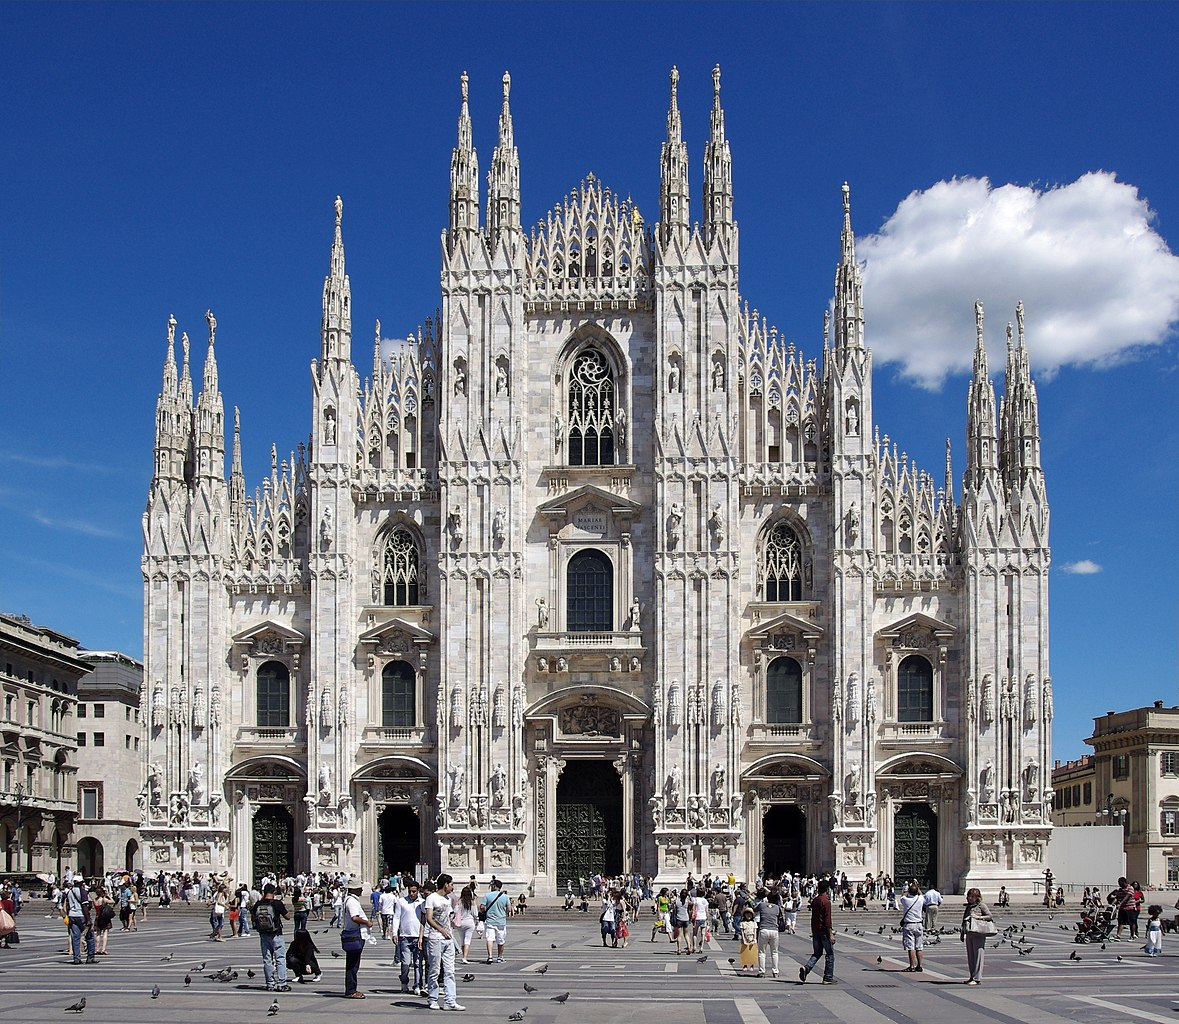
\includegraphics[height=5cm]{figures/milano_old.jpg} }}
    \subfloat{{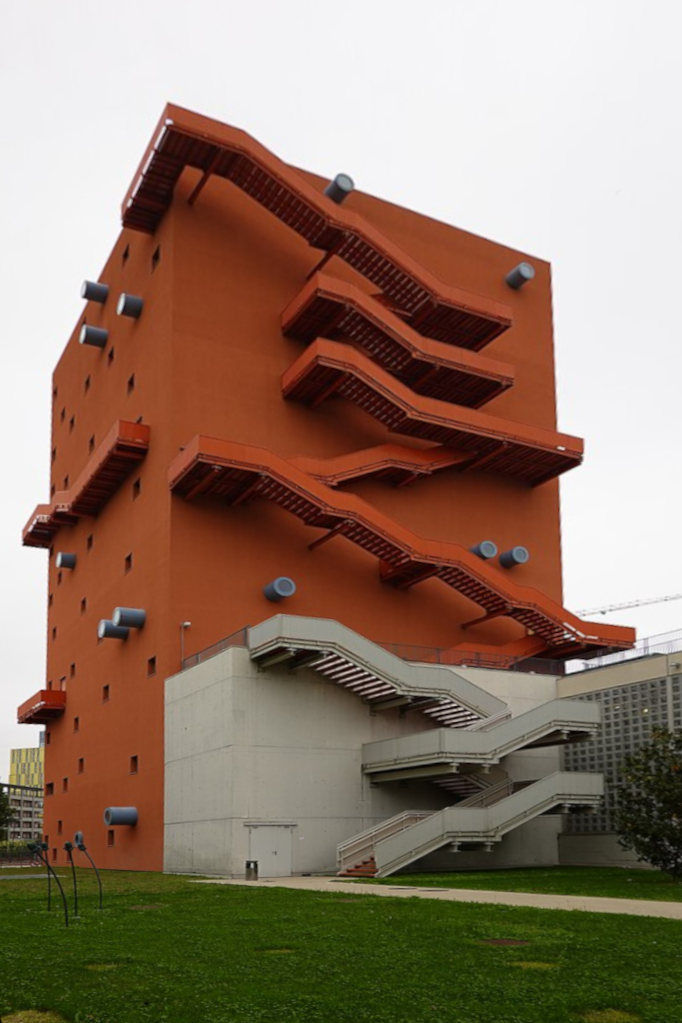
\includegraphics[height=5cm]{figures/milano_ugly.jpg} }}
    \subfloat{{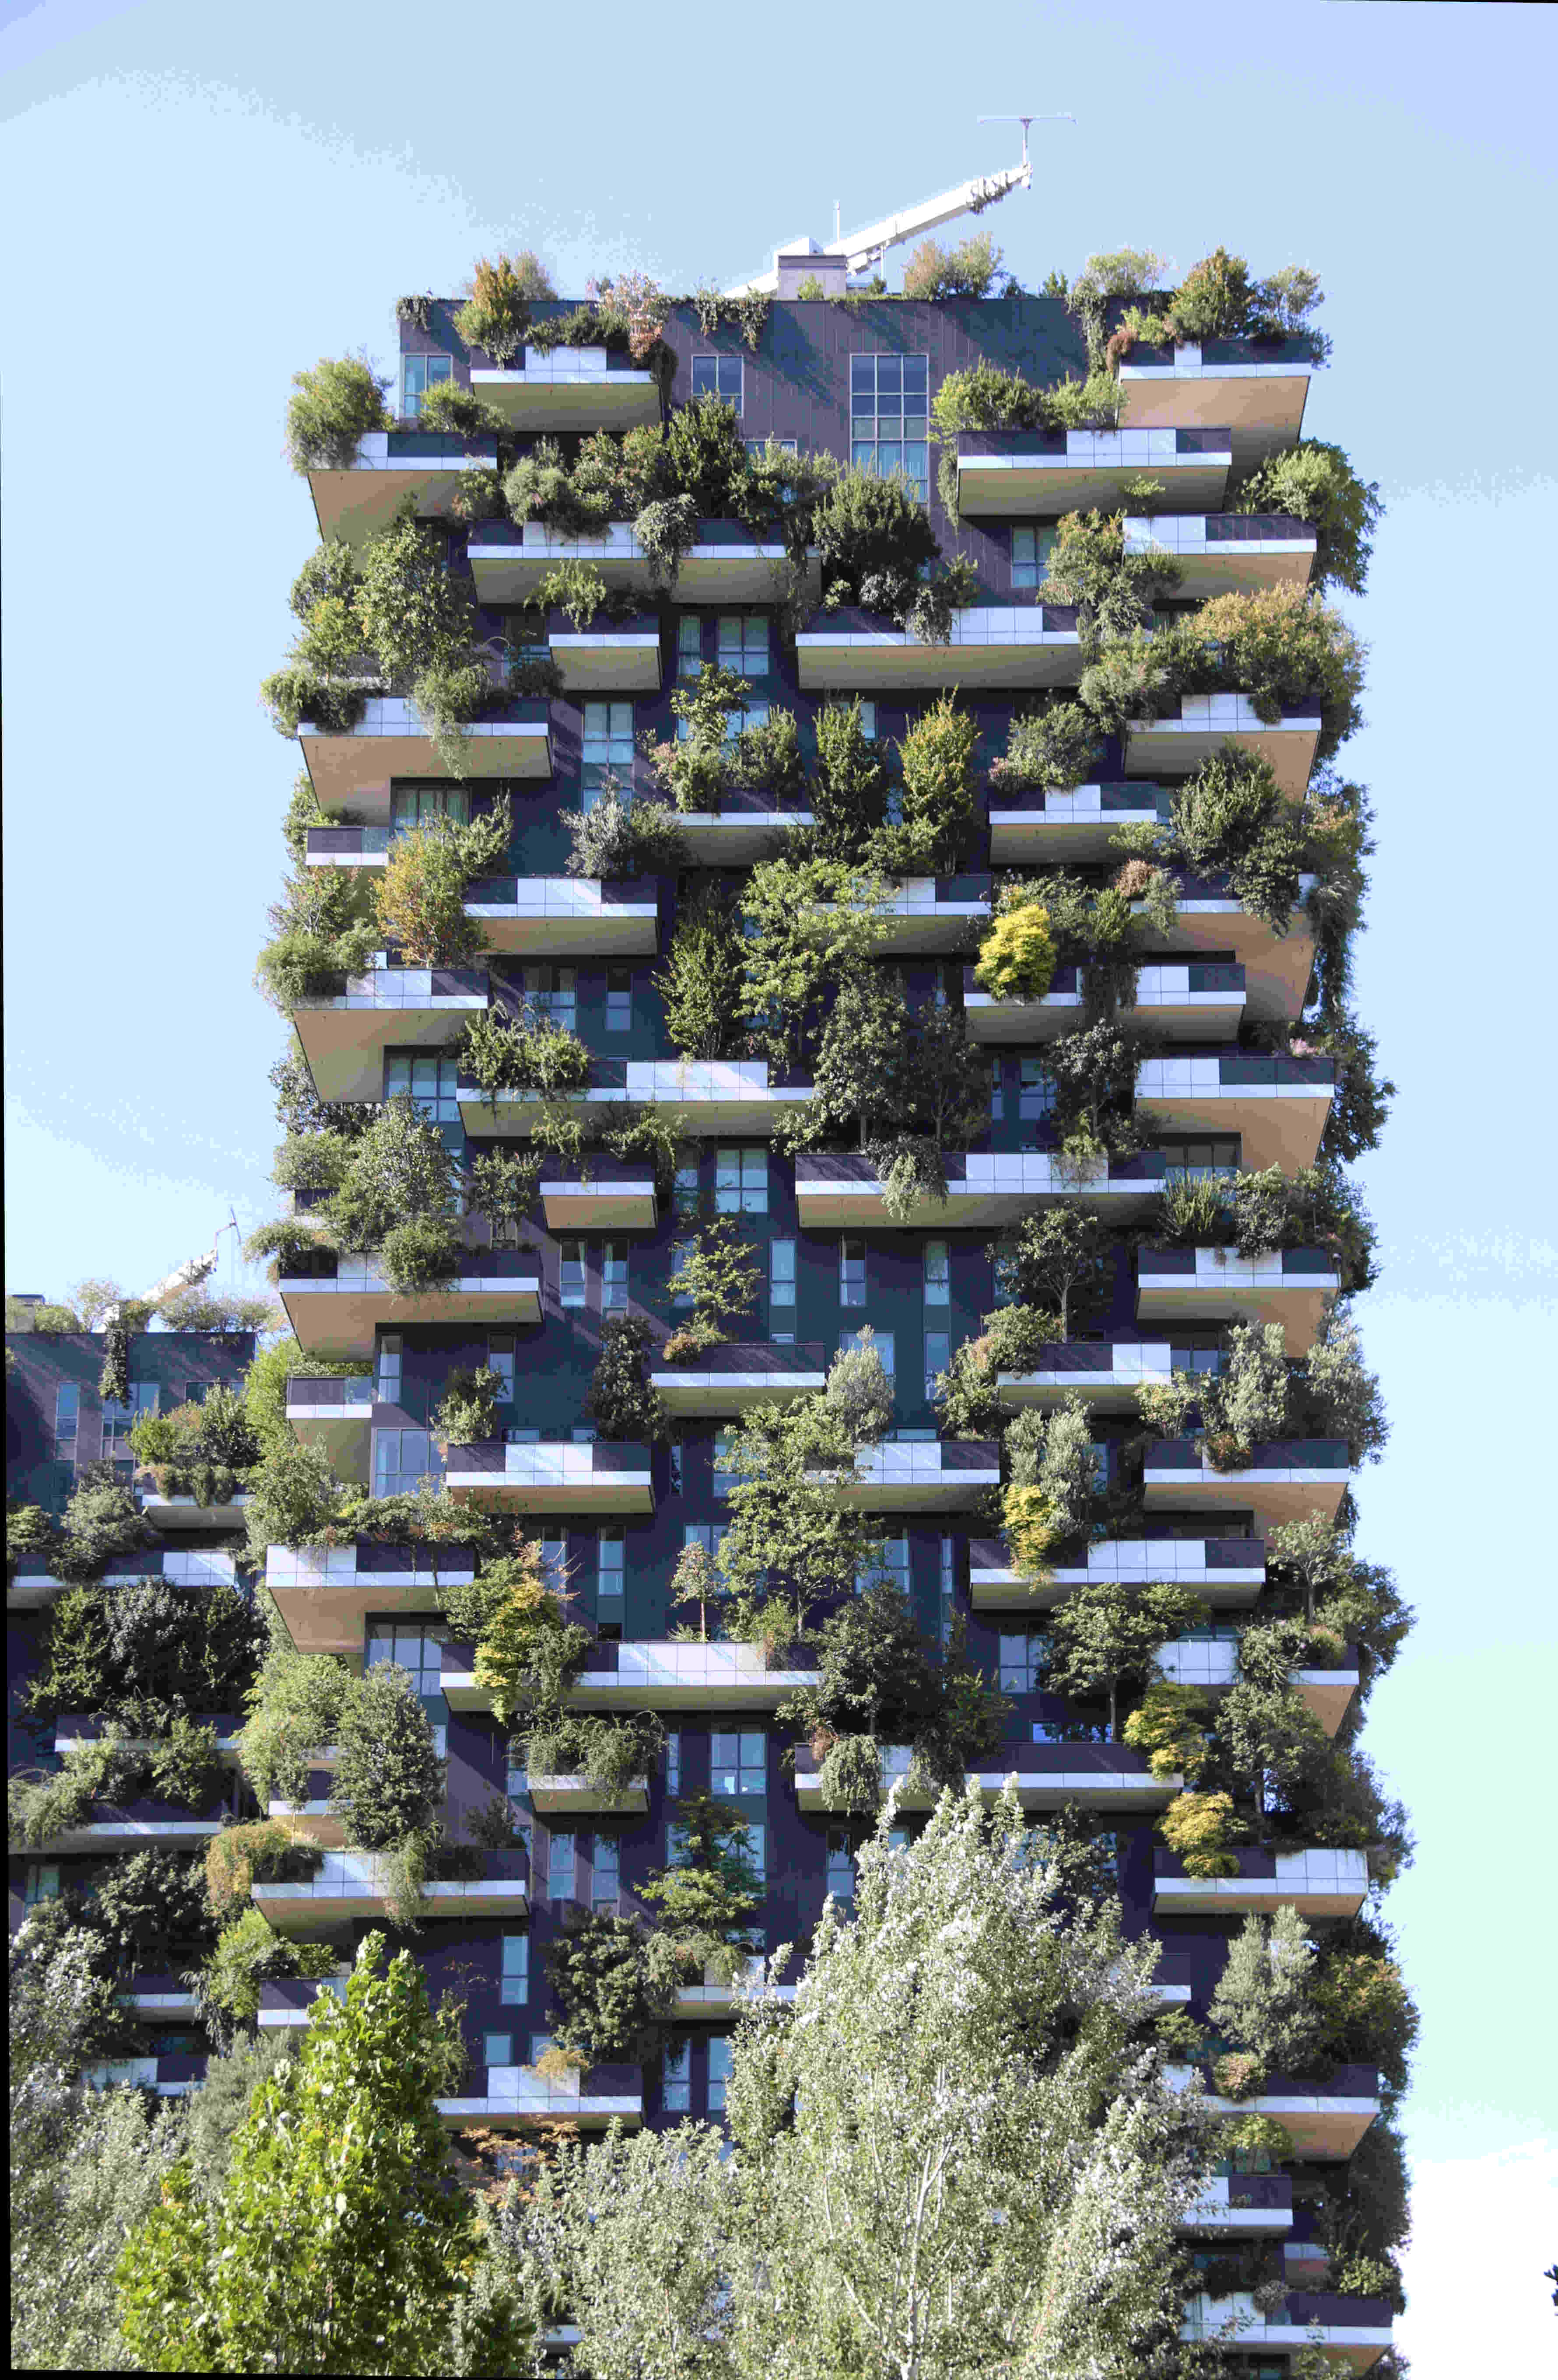
\includegraphics[height=5cm]{figures/milano_biophilic.jpg} }}
    \caption{A selection of well-known buildings from Milan (Italy), neatly representing the thematic arc we laid out in this proposal: From traditional via modernist/brutalist to biophilic architecture. From left to right: Main facade of Milan Cathedral, designed by Simone da Orsenigo in the 14$^\text{th}$ century, a widely recognized landmark of the city. High-rise structure housing part of the design school at the private \textit{IULM University of Milan}, designed by architects of the firm 5+1AAAlfonsoFemiaGianlucaPeluffo in 2014 (\textit{"a design school, you say..?"}). "Bosco Verticale" (en.: vertical forest), one of two residential high-rises designed in 2009 by Stefano Boeri and colleagues. It has been described as \textit{"A house for trees inhabited by humans"} by the architect \cite{noauthor_bosco_2023}. Which of these will score highest on a neurology-based metric for aesthetic experience? We hope to find out! \newline Image sources (left to right): \cite{halun_facade_2011}, \cite{weinold_iulm_2023}, \cite{wikimedia_commons_user_frdr_bosco_2023}}
    \label{fig:sagrada}
\end{figure}

\begin{comment}

\begin{figure}
    \centering
    \subfloat{{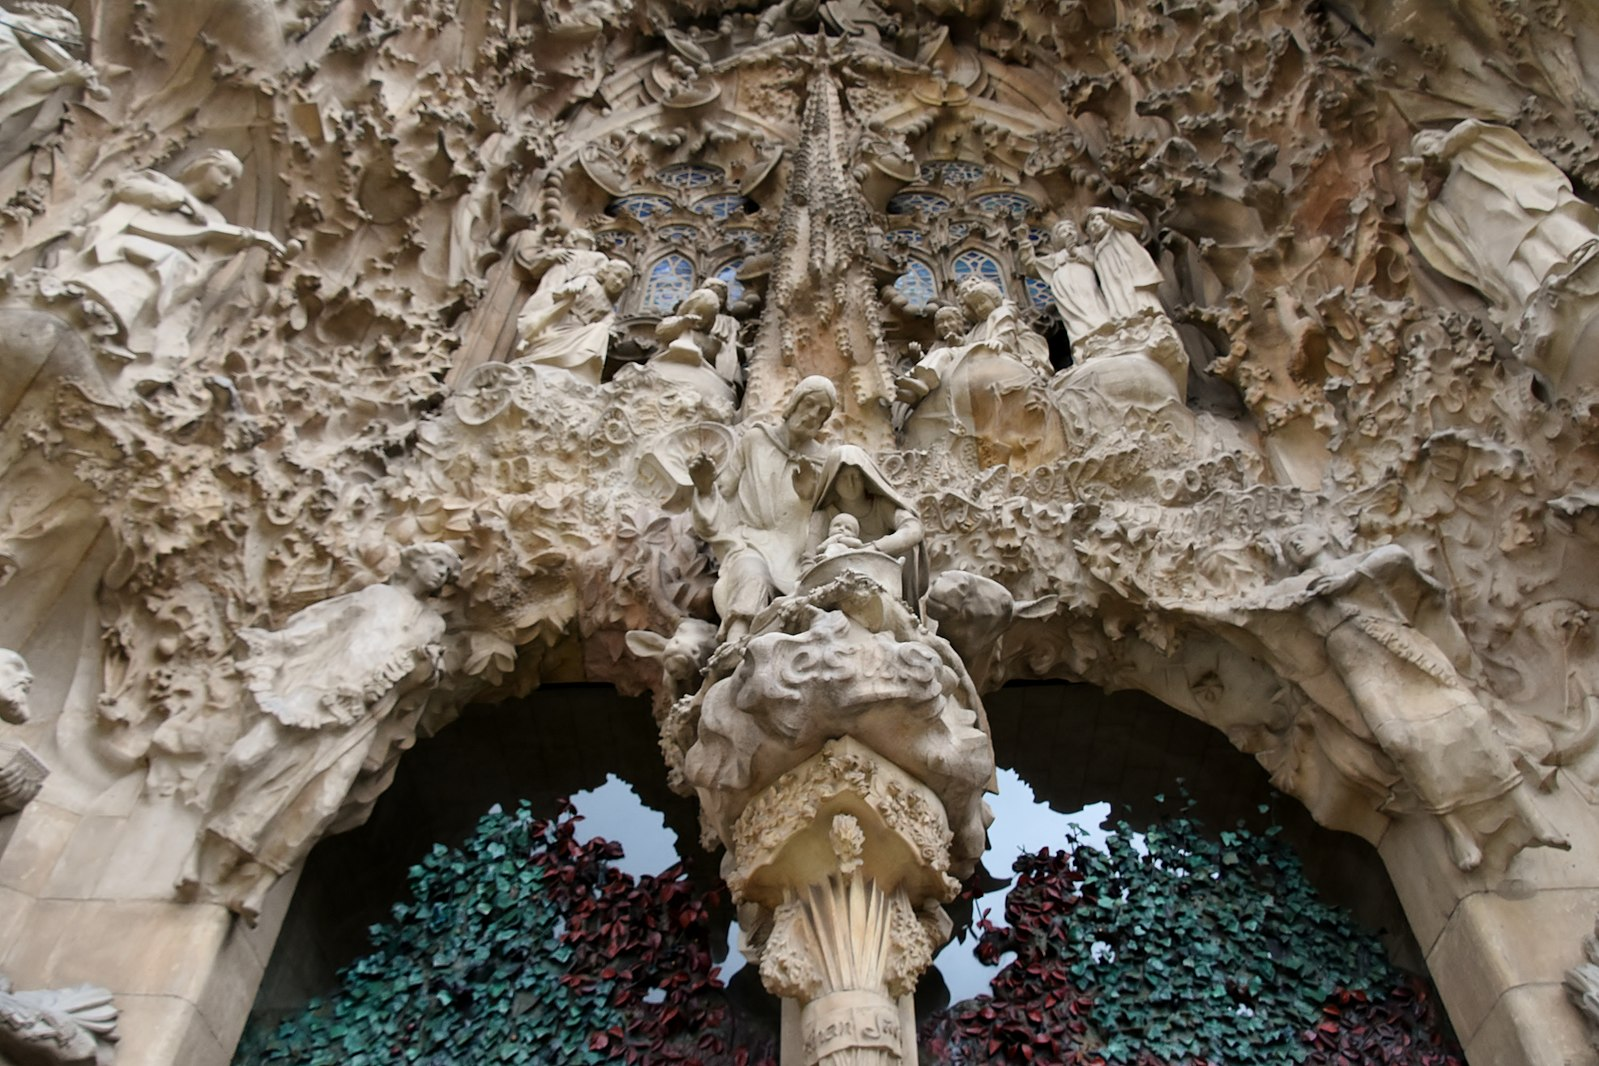
\includegraphics[height=4.75cm]{figures/sagrada_facade.jpg} }}
    \subfloat{{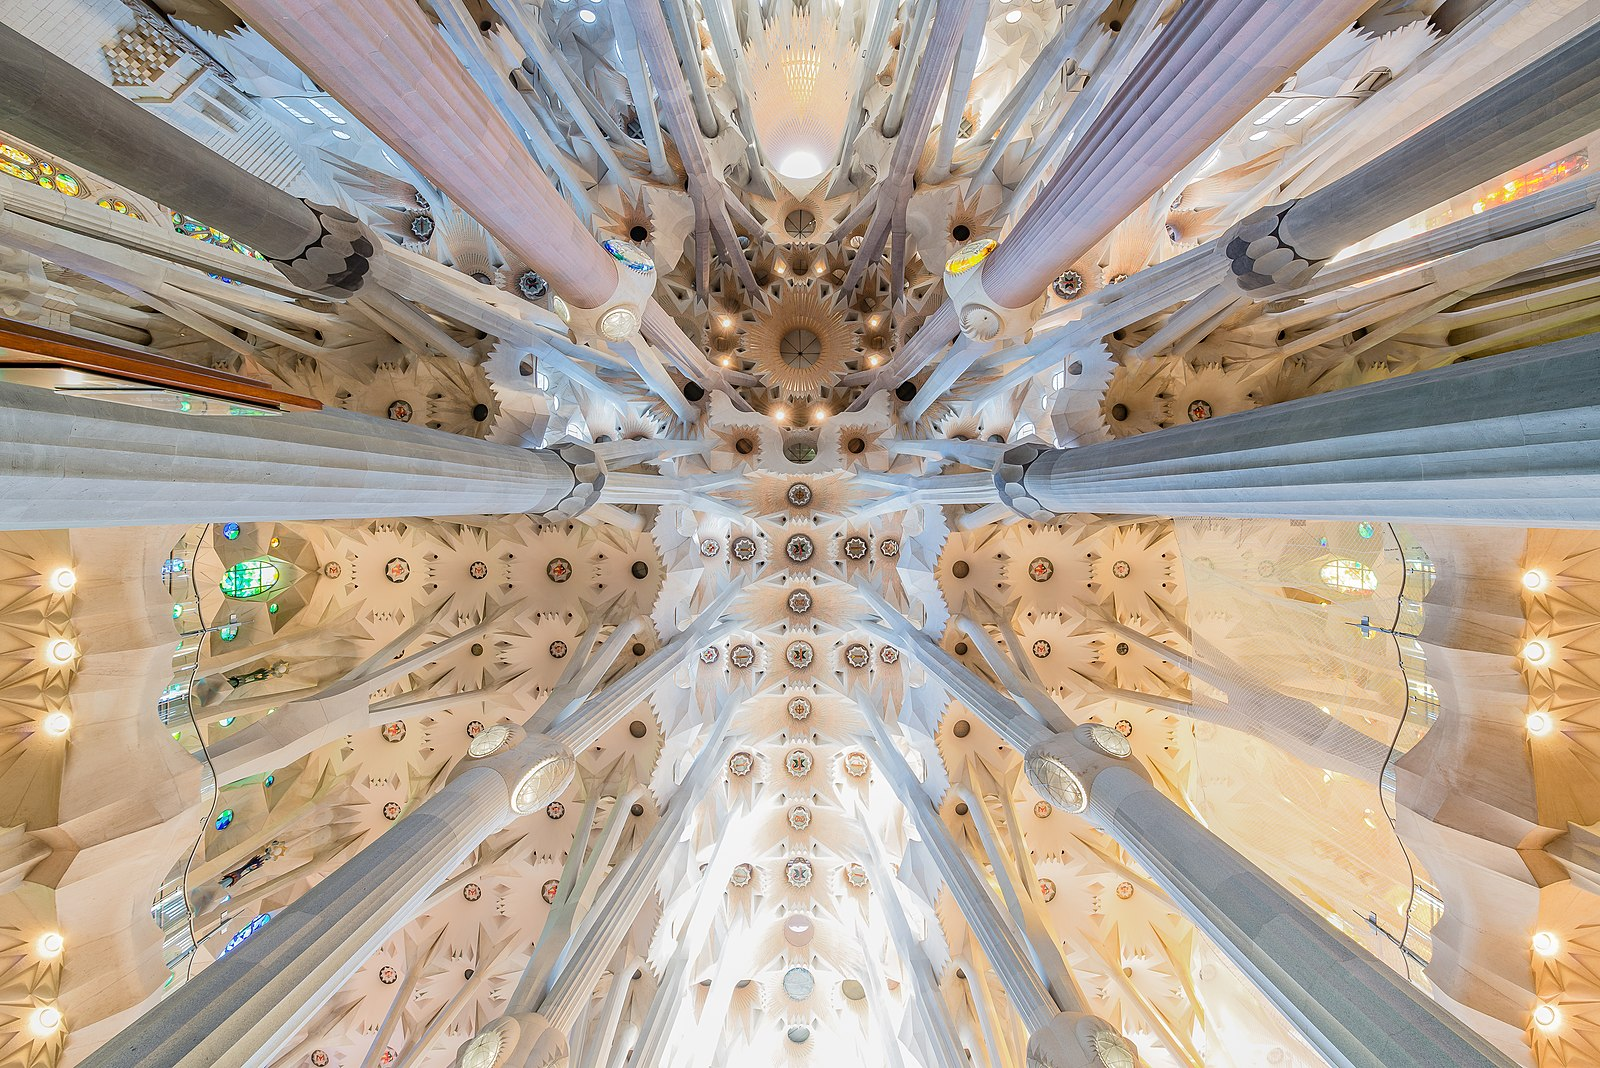
\includegraphics[height=4.75cm]{figures/sagrada_interior.jpg} }}
    \caption{Exterior and interior views of the Gothic Revival/Art Nouveau/Modernista style Catholic church \textit{Sagrada Familia} (en.: "Holy Family") in Barcelona, Spain, designed by Antoni Gaudí from 1883 until his death in 1926. Left: Details of the ornament-laden archway above the main gate of the nativity facade. Right: Wide-angle view of the arboreal load-bearing pillars in the nave. \newline Image sources (left to right): \cite{mortel_sagrada_2016}, \cite{wikimedia_commons_user_t_meltzer_sagrada_2014}.}
    \label{fig:sagrada}
\end{figure}

\begin{figure}
    \centering
    \subfloat{{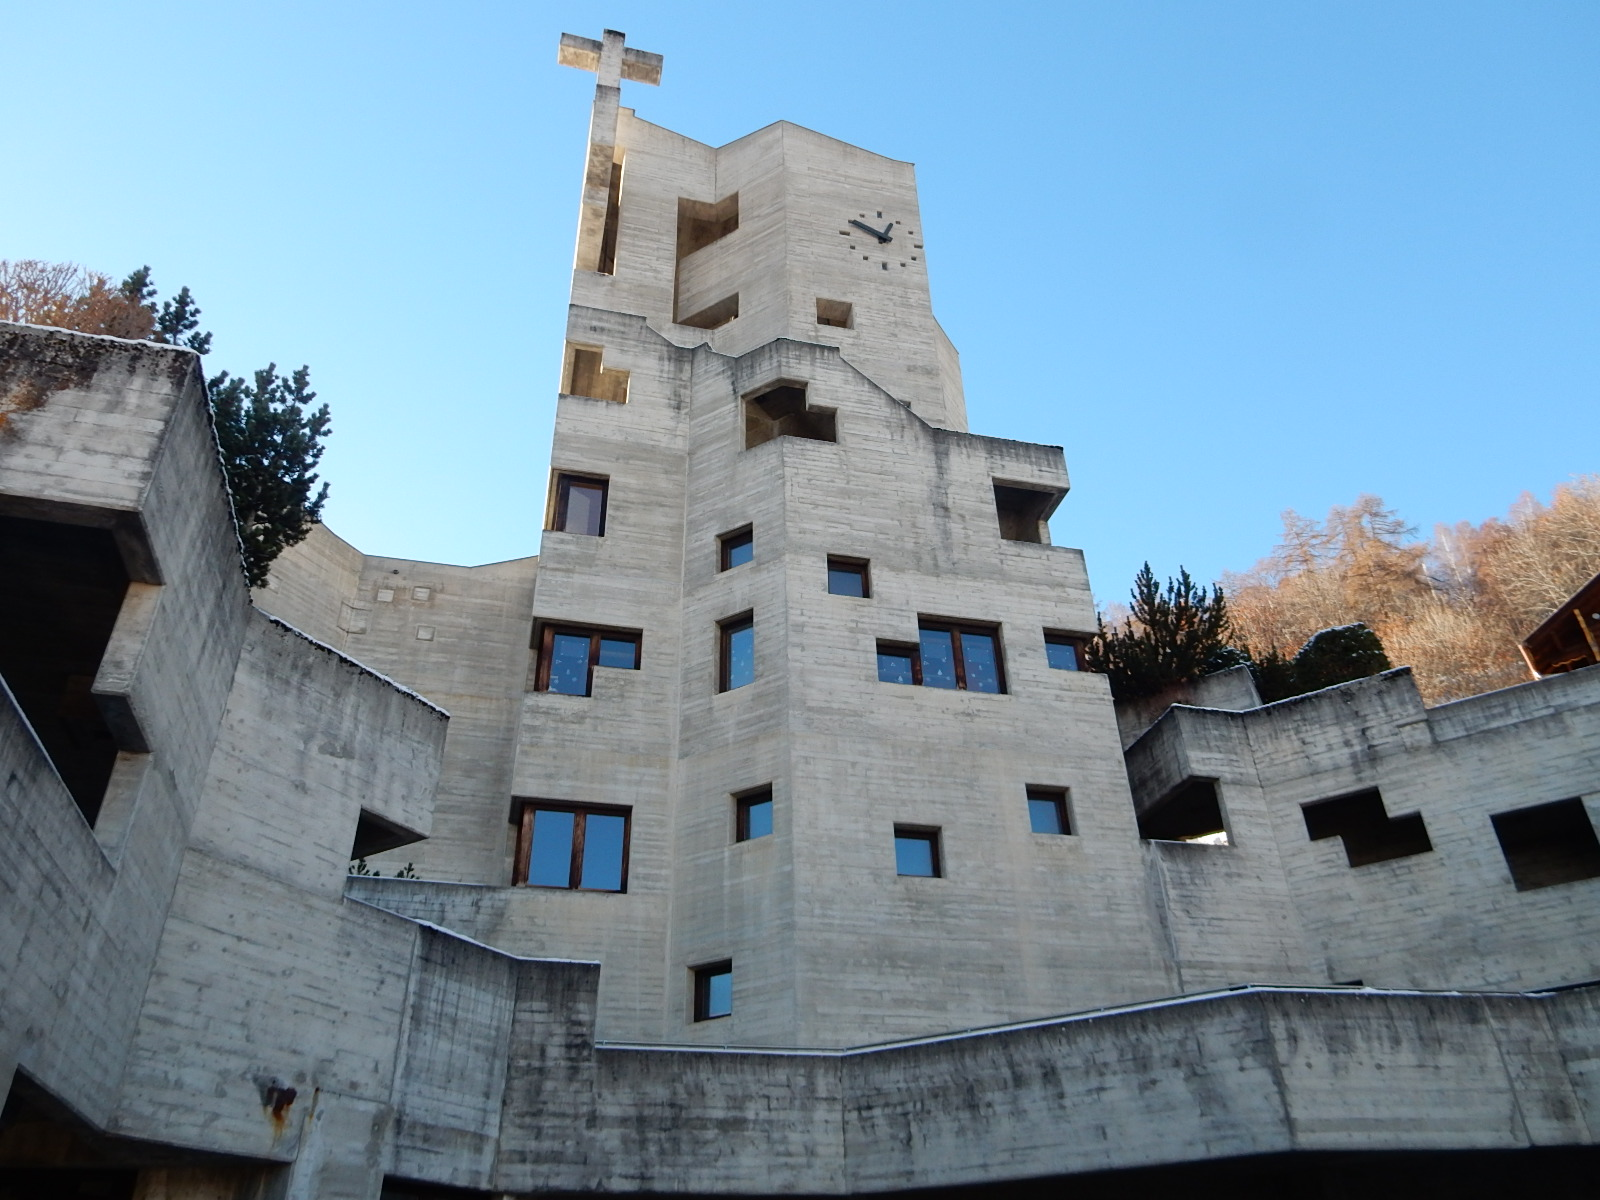
\includegraphics[height=4.5cm]{figures/hérémence_1.jpg} }}
    \subfloat{{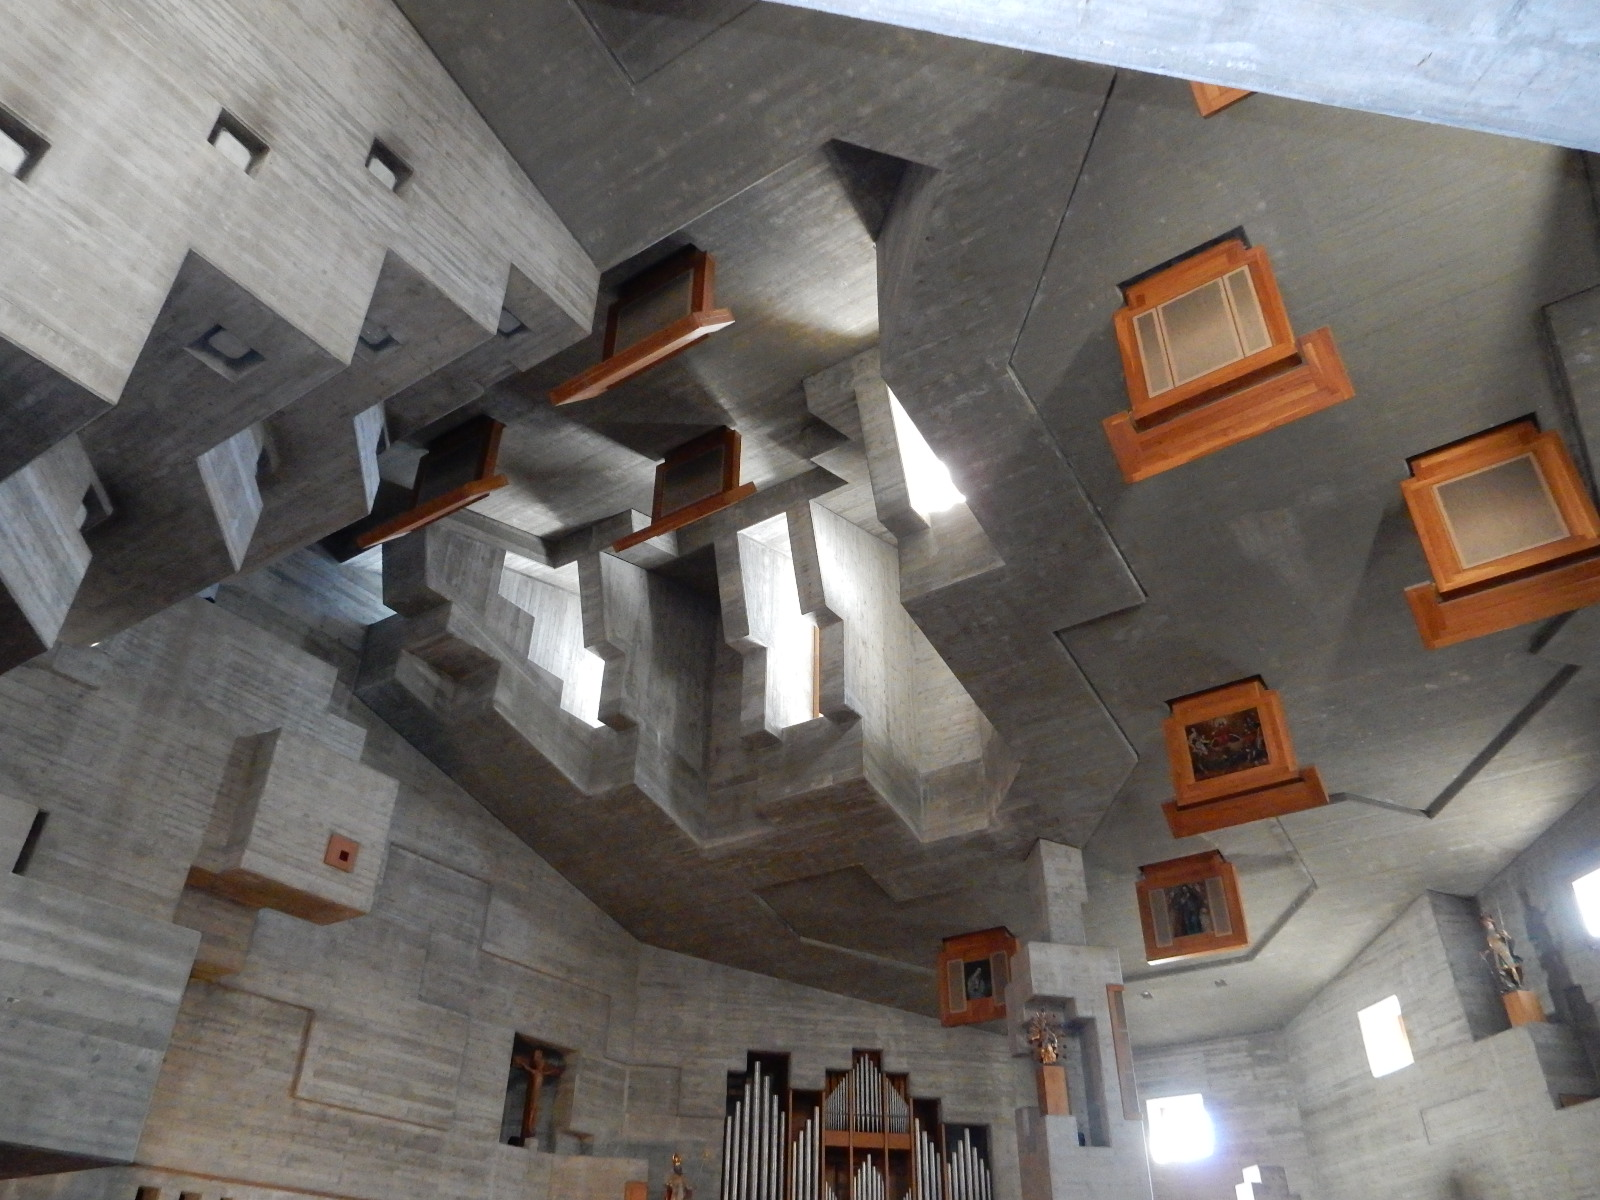
\includegraphics[height=4.5cm]{figures/hérémence_2.jpg} }}
    \caption{Brutalist-style catholic church "St. Nicolas" in the Swiss mountain village of Hérémence, designed by Walter Maria Förderer in 1967. Image sources from left to right: Outside view \cite{bissegger_eglise_2018-1} and inside view \cite{bissegger_eglise_2018}.}
    \label{fig:kunstformen}
\end{figure}

\end{comment}

\clearpage
\printbibliography

\end{document}